\documentclass[11pt]{article}
\renewcommand{\arraystretch}{1.5} % Default value: 1
\usepackage{sectsty}
\allsectionsfont{\color{blue}\fontfamily{lmss}\selectfont}
\usepackage{fontspec}
\setmainfont{XCharter}

\usepackage{listings}
\lstset{
basicstyle=\small\ttfamily,
tabsize=8,
columns=flexible,
breaklines=true,
frame=tb,
rulecolor=\color[rgb]{0.8,0.8,0.7},
backgroundcolor=\color[rgb]{1,1,0.91},
postbreak=\raisebox{0ex}[0ex][0ex]{\ensuremath{\color{red}\hookrightarrow\space}}
}
\usepackage{fontawesome}


\usepackage{mdframed}
\newmdenv[
  backgroundcolor=gray,
  fontcolor=white,
  nobreak=true,
]{terminalinput}



\usepackage{parskip}


    \usepackage[breakable]{tcolorbox}
    \usepackage{parskip} % Stop auto-indenting (to mimic markdown behaviour)

    \usepackage{iftex}
    \ifPDFTeX
    	\usepackage[T1]{fontenc}
    	\usepackage{mathpazo}
    \else
    	\usepackage{fontspec}
    \fi

    % Basic figure setup, for now with no caption control since it's done
    % automatically by Pandoc (which extracts ![](path) syntax from Markdown).
    \usepackage{graphicx}
    % Maintain compatibility with old templates. Remove in nbconvert 6.0
    \let\Oldincludegraphics\includegraphics
    % Ensure that by default, figures have no caption (until we provide a
    % proper Figure object with a Caption API and a way to capture that
    % in the conversion process - todo).
    \usepackage{caption}
    \DeclareCaptionFormat{nocaption}{}
    \captionsetup{labelformat=nolabel, textfont=bf}

    \usepackage[Export]{adjustbox} % Used to constrain images to a maximum size
    \adjustboxset{max size={0.9\linewidth}{0.9\paperheight}}
    \usepackage{float}
    \floatplacement{figure}{H} % forces figures to be placed at the correct location
    \usepackage{xcolor} % Allow colors to be defined
    \usepackage{enumerate} % Needed for markdown enumerations to work
    \usepackage{geometry} % Used to adjust the document margins
    \usepackage{amsmath} % Equations
    \usepackage{amssymb} % Equations
    \usepackage{textcomp} % defines textquotesingle
    % Hack from http://tex.stackexchange.com/a/47451/13684:
    \AtBeginDocument{%
        \def\PYZsq{\textquotesingle}% Upright quotes in Pygmentized code
    }
    \usepackage{upquote} % Upright quotes for verbatim code
    \usepackage{eurosym} % defines \euro
    \usepackage[mathletters]{ucs} % Extended unicode (utf-8) support
    \usepackage{fancyvrb} % verbatim replacement that allows latex
    \usepackage{grffile} % extends the file name processing of package graphics
                         % to support a larger range
    \makeatletter % fix for grffile with XeLaTeX
    \def\Gread@@xetex#1{%
      \IfFileExists{"\Gin@base".bb}%
      {\Gread@eps{\Gin@base.bb}}%
      {\Gread@@xetex@aux#1}%
    }
    \makeatother

    % The hyperref package gives us a pdf with properly built
    % internal navigation ('pdf bookmarks' for the table of contents,
    % internal cross-reference links, web links for URLs, etc.)
    \usepackage{hyperref}
    % The default LaTeX title has an obnoxious amount of whitespace. By default,
    % titling removes some of it. It also provides customization options.
    \usepackage{titling}
    \usepackage{longtable} % longtable support required by pandoc >1.10
    \usepackage{booktabs}  % table support for pandoc > 1.12.2
    \usepackage[inline]{enumitem} % IRkernel/repr support (it uses the enumerate* environment)
    \usepackage[normalem]{ulem} % ulem is needed to support strikethroughs (\sout)
                                % normalem makes italics be italics, not underlines
    \usepackage{mathrsfs}



    % Colors for the hyperref package
    \definecolor{urlcolor}{rgb}{0,.145,.698}
    \definecolor{linkcolor}{rgb}{.71,0.21,0.01}
    \definecolor{citecolor}{rgb}{.12,.54,.11}

    % ANSI colors
    \definecolor{ansi-black}{HTML}{3E424D}
    \definecolor{ansi-black-intense}{HTML}{282C36}
    \definecolor{ansi-red}{HTML}{E75C58}
    \definecolor{ansi-red-intense}{HTML}{B22B31}
    \definecolor{ansi-green}{HTML}{00A250}
    \definecolor{ansi-green-intense}{HTML}{007427}
    \definecolor{ansi-yellow}{HTML}{DDB62B}
    \definecolor{ansi-yellow-intense}{HTML}{B27D12}
    \definecolor{ansi-blue}{HTML}{208FFB}
    \definecolor{ansi-blue-intense}{HTML}{0065CA}
    \definecolor{ansi-magenta}{HTML}{D160C4}
    \definecolor{ansi-magenta-intense}{HTML}{A03196}
    \definecolor{ansi-cyan}{HTML}{60C6C8}
    \definecolor{ansi-cyan-intense}{HTML}{258F8F}
    \definecolor{ansi-white}{HTML}{C5C1B4}
    \definecolor{ansi-white-intense}{HTML}{A1A6B2}
    \definecolor{ansi-default-inverse-fg}{HTML}{FFFFFF}
    \definecolor{ansi-default-inverse-bg}{HTML}{000000}

    % commands and environments needed by pandoc snippets
    % extracted from the output of `pandoc -s`
    \providecommand{\tightlist}{%
      \setlength{\itemsep}{0pt}\setlength{\parskip}{0pt}}
    \DefineVerbatimEnvironment{Highlighting}{Verbatim}{commandchars=\\\{\}}
    % Add ',fontsize=\small' for more characters per line
    \newenvironment{Shaded}{}{}
    \newcommand{\KeywordTok}[1]{\textcolor[rgb]{0.00,0.44,0.13}{\textbf{{#1}}}}
    \newcommand{\DataTypeTok}[1]{\textcolor[rgb]{0.56,0.13,0.00}{{#1}}}
    \newcommand{\DecValTok}[1]{\textcolor[rgb]{0.25,0.63,0.44}{{#1}}}
    \newcommand{\BaseNTok}[1]{\textcolor[rgb]{0.25,0.63,0.44}{{#1}}}
    \newcommand{\FloatTok}[1]{\textcolor[rgb]{0.25,0.63,0.44}{{#1}}}
    \newcommand{\CharTok}[1]{\textcolor[rgb]{0.25,0.44,0.63}{{#1}}}
    \newcommand{\StringTok}[1]{\textcolor[rgb]{0.25,0.44,0.63}{{#1}}}
    \newcommand{\CommentTok}[1]{\textcolor[rgb]{0.38,0.63,0.69}{\textit{{#1}}}}
    \newcommand{\OtherTok}[1]{\textcolor[rgb]{0.00,0.44,0.13}{{#1}}}
    \newcommand{\AlertTok}[1]{\textcolor[rgb]{1.00,0.00,0.00}{\textbf{{#1}}}}
    \newcommand{\FunctionTok}[1]{\textcolor[rgb]{0.02,0.16,0.49}{{#1}}}
    \newcommand{\RegionMarkerTok}[1]{{#1}}
    \newcommand{\ErrorTok}[1]{\textcolor[rgb]{1.00,0.00,0.00}{\textbf{{#1}}}}
    \newcommand{\NormalTok}[1]{{#1}}

    % Additional commands for more recent versions of Pandoc
    \newcommand{\ConstantTok}[1]{\textcolor[rgb]{0.53,0.00,0.00}{{#1}}}
    \newcommand{\SpecialCharTok}[1]{\textcolor[rgb]{0.25,0.44,0.63}{{#1}}}
    \newcommand{\VerbatimStringTok}[1]{\textcolor[rgb]{0.25,0.44,0.63}{{#1}}}
    \newcommand{\SpecialStringTok}[1]{\textcolor[rgb]{0.73,0.40,0.53}{{#1}}}
    \newcommand{\ImportTok}[1]{{#1}}
    \newcommand{\DocumentationTok}[1]{\textcolor[rgb]{0.73,0.13,0.13}{\textit{{#1}}}}
    \newcommand{\AnnotationTok}[1]{\textcolor[rgb]{0.38,0.63,0.69}{\textbf{\textit{{#1}}}}}
    \newcommand{\CommentVarTok}[1]{\textcolor[rgb]{0.38,0.63,0.69}{\textbf{\textit{{#1}}}}}
    \newcommand{\VariableTok}[1]{\textcolor[rgb]{0.10,0.09,0.49}{{#1}}}
    \newcommand{\ControlFlowTok}[1]{\textcolor[rgb]{0.00,0.44,0.13}{\textbf{{#1}}}}
    \newcommand{\OperatorTok}[1]{\textcolor[rgb]{0.40,0.40,0.40}{{#1}}}
    \newcommand{\BuiltInTok}[1]{{#1}}
    \newcommand{\ExtensionTok}[1]{{#1}}
    \newcommand{\PreprocessorTok}[1]{\textcolor[rgb]{0.74,0.48,0.00}{{#1}}}
    \newcommand{\AttributeTok}[1]{\textcolor[rgb]{0.49,0.56,0.16}{{#1}}}
    \newcommand{\InformationTok}[1]{\textcolor[rgb]{0.38,0.63,0.69}{\textbf{\textit{{#1}}}}}
    \newcommand{\WarningTok}[1]{\textcolor[rgb]{0.38,0.63,0.69}{\textbf{\textit{{#1}}}}}


    % Define a nice break command that doesn't care if a line doesn't already
    % exist.
    \def\br{\hspace*{\fill} \\* }
    % Math Jax compatibility definitions
    \def\gt{>}
    \def\lt{<}
    \let\Oldtex\TeX
    \let\Oldlatex\LaTeX
    \renewcommand{\TeX}{\textrm{\Oldtex}}
    \renewcommand{\LaTeX}{\textrm{\Oldlatex}}
    % Document parameters
    % Document title
    \title{index}





% Pygments definitions
\makeatletter
\def\PY@reset{\let\PY@it=\relax \let\PY@bf=\relax%
    \let\PY@ul=\relax \let\PY@tc=\relax%
    \let\PY@bc=\relax \let\PY@ff=\relax}
\def\PY@tok#1{\csname PY@tok@#1\endcsname}
\def\PY@toks#1+{\ifx\relax#1\empty\else%
    \PY@tok{#1}\expandafter\PY@toks\fi}
\def\PY@do#1{\PY@bc{\PY@tc{\PY@ul{%
    \PY@it{\PY@bf{\PY@ff{#1}}}}}}}
\def\PY#1#2{\PY@reset\PY@toks#1+\relax+\PY@do{#2}}

\expandafter\def\csname PY@tok@w\endcsname{\def\PY@tc##1{\textcolor[rgb]{0.73,0.73,0.73}{##1}}}
\expandafter\def\csname PY@tok@c\endcsname{\let\PY@it=\textit\def\PY@tc##1{\textcolor[rgb]{0.25,0.50,0.50}{##1}}}
\expandafter\def\csname PY@tok@cp\endcsname{\def\PY@tc##1{\textcolor[rgb]{0.74,0.48,0.00}{##1}}}
\expandafter\def\csname PY@tok@k\endcsname{\let\PY@bf=\textbf\def\PY@tc##1{\textcolor[rgb]{0.00,0.50,0.00}{##1}}}
\expandafter\def\csname PY@tok@kp\endcsname{\def\PY@tc##1{\textcolor[rgb]{0.00,0.50,0.00}{##1}}}
\expandafter\def\csname PY@tok@kt\endcsname{\def\PY@tc##1{\textcolor[rgb]{0.69,0.00,0.25}{##1}}}
\expandafter\def\csname PY@tok@o\endcsname{\def\PY@tc##1{\textcolor[rgb]{0.40,0.40,0.40}{##1}}}
\expandafter\def\csname PY@tok@ow\endcsname{\let\PY@bf=\textbf\def\PY@tc##1{\textcolor[rgb]{0.67,0.13,1.00}{##1}}}
\expandafter\def\csname PY@tok@nb\endcsname{\def\PY@tc##1{\textcolor[rgb]{0.00,0.50,0.00}{##1}}}
\expandafter\def\csname PY@tok@nf\endcsname{\def\PY@tc##1{\textcolor[rgb]{0.00,0.00,1.00}{##1}}}
\expandafter\def\csname PY@tok@nc\endcsname{\let\PY@bf=\textbf\def\PY@tc##1{\textcolor[rgb]{0.00,0.00,1.00}{##1}}}
\expandafter\def\csname PY@tok@nn\endcsname{\let\PY@bf=\textbf\def\PY@tc##1{\textcolor[rgb]{0.00,0.00,1.00}{##1}}}
\expandafter\def\csname PY@tok@ne\endcsname{\let\PY@bf=\textbf\def\PY@tc##1{\textcolor[rgb]{0.82,0.25,0.23}{##1}}}
\expandafter\def\csname PY@tok@nv\endcsname{\def\PY@tc##1{\textcolor[rgb]{0.10,0.09,0.49}{##1}}}
\expandafter\def\csname PY@tok@no\endcsname{\def\PY@tc##1{\textcolor[rgb]{0.53,0.00,0.00}{##1}}}
\expandafter\def\csname PY@tok@nl\endcsname{\def\PY@tc##1{\textcolor[rgb]{0.63,0.63,0.00}{##1}}}
\expandafter\def\csname PY@tok@ni\endcsname{\let\PY@bf=\textbf\def\PY@tc##1{\textcolor[rgb]{0.60,0.60,0.60}{##1}}}
\expandafter\def\csname PY@tok@na\endcsname{\def\PY@tc##1{\textcolor[rgb]{0.49,0.56,0.16}{##1}}}
\expandafter\def\csname PY@tok@nt\endcsname{\let\PY@bf=\textbf\def\PY@tc##1{\textcolor[rgb]{0.00,0.50,0.00}{##1}}}
\expandafter\def\csname PY@tok@nd\endcsname{\def\PY@tc##1{\textcolor[rgb]{0.67,0.13,1.00}{##1}}}
\expandafter\def\csname PY@tok@s\endcsname{\def\PY@tc##1{\textcolor[rgb]{0.73,0.13,0.13}{##1}}}
\expandafter\def\csname PY@tok@sd\endcsname{\let\PY@it=\textit\def\PY@tc##1{\textcolor[rgb]{0.73,0.13,0.13}{##1}}}
\expandafter\def\csname PY@tok@si\endcsname{\let\PY@bf=\textbf\def\PY@tc##1{\textcolor[rgb]{0.73,0.40,0.53}{##1}}}
\expandafter\def\csname PY@tok@se\endcsname{\let\PY@bf=\textbf\def\PY@tc##1{\textcolor[rgb]{0.73,0.40,0.13}{##1}}}
\expandafter\def\csname PY@tok@sr\endcsname{\def\PY@tc##1{\textcolor[rgb]{0.73,0.40,0.53}{##1}}}
\expandafter\def\csname PY@tok@ss\endcsname{\def\PY@tc##1{\textcolor[rgb]{0.10,0.09,0.49}{##1}}}
\expandafter\def\csname PY@tok@sx\endcsname{\def\PY@tc##1{\textcolor[rgb]{0.00,0.50,0.00}{##1}}}
\expandafter\def\csname PY@tok@m\endcsname{\def\PY@tc##1{\textcolor[rgb]{0.40,0.40,0.40}{##1}}}
\expandafter\def\csname PY@tok@gh\endcsname{\let\PY@bf=\textbf\def\PY@tc##1{\textcolor[rgb]{0.00,0.00,0.50}{##1}}}
\expandafter\def\csname PY@tok@gu\endcsname{\let\PY@bf=\textbf\def\PY@tc##1{\textcolor[rgb]{0.50,0.00,0.50}{##1}}}
\expandafter\def\csname PY@tok@gd\endcsname{\def\PY@tc##1{\textcolor[rgb]{0.63,0.00,0.00}{##1}}}
\expandafter\def\csname PY@tok@gi\endcsname{\def\PY@tc##1{\textcolor[rgb]{0.00,0.63,0.00}{##1}}}
\expandafter\def\csname PY@tok@gr\endcsname{\def\PY@tc##1{\textcolor[rgb]{1.00,0.00,0.00}{##1}}}
\expandafter\def\csname PY@tok@ge\endcsname{\let\PY@it=\textit}
\expandafter\def\csname PY@tok@gs\endcsname{\let\PY@bf=\textbf}
\expandafter\def\csname PY@tok@gp\endcsname{\let\PY@bf=\textbf\def\PY@tc##1{\textcolor[rgb]{0.00,0.00,0.50}{##1}}}
\expandafter\def\csname PY@tok@go\endcsname{\def\PY@tc##1{\textcolor[rgb]{0.53,0.53,0.53}{##1}}}
\expandafter\def\csname PY@tok@gt\endcsname{\def\PY@tc##1{\textcolor[rgb]{0.00,0.27,0.87}{##1}}}
\expandafter\def\csname PY@tok@err\endcsname{\def\PY@bc##1{\setlength{\fboxsep}{0pt}\fcolorbox[rgb]{1.00,0.00,0.00}{1,1,1}{\strut ##1}}}
\expandafter\def\csname PY@tok@kc\endcsname{\let\PY@bf=\textbf\def\PY@tc##1{\textcolor[rgb]{0.00,0.50,0.00}{##1}}}
\expandafter\def\csname PY@tok@kd\endcsname{\let\PY@bf=\textbf\def\PY@tc##1{\textcolor[rgb]{0.00,0.50,0.00}{##1}}}
\expandafter\def\csname PY@tok@kn\endcsname{\let\PY@bf=\textbf\def\PY@tc##1{\textcolor[rgb]{0.00,0.50,0.00}{##1}}}
\expandafter\def\csname PY@tok@kr\endcsname{\let\PY@bf=\textbf\def\PY@tc##1{\textcolor[rgb]{0.00,0.50,0.00}{##1}}}
\expandafter\def\csname PY@tok@bp\endcsname{\def\PY@tc##1{\textcolor[rgb]{0.00,0.50,0.00}{##1}}}
\expandafter\def\csname PY@tok@fm\endcsname{\def\PY@tc##1{\textcolor[rgb]{0.00,0.00,1.00}{##1}}}
\expandafter\def\csname PY@tok@vc\endcsname{\def\PY@tc##1{\textcolor[rgb]{0.10,0.09,0.49}{##1}}}
\expandafter\def\csname PY@tok@vg\endcsname{\def\PY@tc##1{\textcolor[rgb]{0.10,0.09,0.49}{##1}}}
\expandafter\def\csname PY@tok@vi\endcsname{\def\PY@tc##1{\textcolor[rgb]{0.10,0.09,0.49}{##1}}}
\expandafter\def\csname PY@tok@vm\endcsname{\def\PY@tc##1{\textcolor[rgb]{0.10,0.09,0.49}{##1}}}
\expandafter\def\csname PY@tok@sa\endcsname{\def\PY@tc##1{\textcolor[rgb]{0.73,0.13,0.13}{##1}}}
\expandafter\def\csname PY@tok@sb\endcsname{\def\PY@tc##1{\textcolor[rgb]{0.73,0.13,0.13}{##1}}}
\expandafter\def\csname PY@tok@sc\endcsname{\def\PY@tc##1{\textcolor[rgb]{0.73,0.13,0.13}{##1}}}
\expandafter\def\csname PY@tok@dl\endcsname{\def\PY@tc##1{\textcolor[rgb]{0.73,0.13,0.13}{##1}}}
\expandafter\def\csname PY@tok@s2\endcsname{\def\PY@tc##1{\textcolor[rgb]{0.73,0.13,0.13}{##1}}}
\expandafter\def\csname PY@tok@sh\endcsname{\def\PY@tc##1{\textcolor[rgb]{0.73,0.13,0.13}{##1}}}
\expandafter\def\csname PY@tok@s1\endcsname{\def\PY@tc##1{\textcolor[rgb]{0.73,0.13,0.13}{##1}}}
\expandafter\def\csname PY@tok@mb\endcsname{\def\PY@tc##1{\textcolor[rgb]{0.40,0.40,0.40}{##1}}}
\expandafter\def\csname PY@tok@mf\endcsname{\def\PY@tc##1{\textcolor[rgb]{0.40,0.40,0.40}{##1}}}
\expandafter\def\csname PY@tok@mh\endcsname{\def\PY@tc##1{\textcolor[rgb]{0.40,0.40,0.40}{##1}}}
\expandafter\def\csname PY@tok@mi\endcsname{\def\PY@tc##1{\textcolor[rgb]{0.40,0.40,0.40}{##1}}}
\expandafter\def\csname PY@tok@il\endcsname{\def\PY@tc##1{\textcolor[rgb]{0.40,0.40,0.40}{##1}}}
\expandafter\def\csname PY@tok@mo\endcsname{\def\PY@tc##1{\textcolor[rgb]{0.40,0.40,0.40}{##1}}}
\expandafter\def\csname PY@tok@ch\endcsname{\let\PY@it=\textit\def\PY@tc##1{\textcolor[rgb]{0.25,0.50,0.50}{##1}}}
\expandafter\def\csname PY@tok@cm\endcsname{\let\PY@it=\textit\def\PY@tc##1{\textcolor[rgb]{0.25,0.50,0.50}{##1}}}
\expandafter\def\csname PY@tok@cpf\endcsname{\let\PY@it=\textit\def\PY@tc##1{\textcolor[rgb]{0.25,0.50,0.50}{##1}}}
\expandafter\def\csname PY@tok@c1\endcsname{\let\PY@it=\textit\def\PY@tc##1{\textcolor[rgb]{0.25,0.50,0.50}{##1}}}
\expandafter\def\csname PY@tok@cs\endcsname{\let\PY@it=\textit\def\PY@tc##1{\textcolor[rgb]{0.25,0.50,0.50}{##1}}}

\def\PYZbs{\char`\\}
\def\PYZus{\char`\_}
\def\PYZob{\char`\{}
\def\PYZcb{\char`\}}
\def\PYZca{\char`\^}
\def\PYZam{\char`\&}
\def\PYZlt{\char`\<}
\def\PYZgt{\char`\>}
\def\PYZsh{\char`\#}
\def\PYZpc{\char`\%}
\def\PYZdl{\char`\$}
\def\PYZhy{\char`\-}
\def\PYZsq{\char`\'}
\def\PYZdq{\char`\"}
\def\PYZti{\char`\~}
% for compatibility with earlier versions
\def\PYZat{@}
\def\PYZlb{[}
\def\PYZrb{]}
\makeatother


    % For linebreaks inside Verbatim environment from package fancyvrb.
    \makeatletter
        \newbox\Wrappedcontinuationbox
        \newbox\Wrappedvisiblespacebox
        \newcommand*\Wrappedvisiblespace {\textcolor{red}{\textvisiblespace}}
        \newcommand*\Wrappedcontinuationsymbol {\textcolor{red}{\llap{\tiny$\m@th\hookrightarrow$}}}
        \newcommand*\Wrappedcontinuationindent {3ex }
        \newcommand*\Wrappedafterbreak {\kern\Wrappedcontinuationindent\copy\Wrappedcontinuationbox}
        % Take advantage of the already applied Pygments mark-up to insert
        % potential linebreaks for TeX processing.
        %        {, <, #, %, $, ' and ": go to next line.
        %        _, }, ^, &, >, - and ~: stay at end of broken line.
        % Use of \textquotesingle for straight quote.
        \newcommand*\Wrappedbreaksatspecials {%
            \def\PYGZus{\discretionary{\char`\_}{\Wrappedafterbreak}{\char`\_}}%
            \def\PYGZob{\discretionary{}{\Wrappedafterbreak\char`\{}{\char`\{}}%
            \def\PYGZcb{\discretionary{\char`\}}{\Wrappedafterbreak}{\char`\}}}%
            \def\PYGZca{\discretionary{\char`\^}{\Wrappedafterbreak}{\char`\^}}%
            \def\PYGZam{\discretionary{\char`\&}{\Wrappedafterbreak}{\char`\&}}%
            \def\PYGZlt{\discretionary{}{\Wrappedafterbreak\char`\<}{\char`\<}}%
            \def\PYGZgt{\discretionary{\char`\>}{\Wrappedafterbreak}{\char`\>}}%
            \def\PYGZsh{\discretionary{}{\Wrappedafterbreak\char`\#}{\char`\#}}%
            \def\PYGZpc{\discretionary{}{\Wrappedafterbreak\char`\%}{\char`\%}}%
            \def\PYGZdl{\discretionary{}{\Wrappedafterbreak\char`\$}{\char`\$}}%
            \def\PYGZhy{\discretionary{\char`\-}{\Wrappedafterbreak}{\char`\-}}%
            \def\PYGZsq{\discretionary{}{\Wrappedafterbreak\textquotesingle}{\textquotesingle}}%
            \def\PYGZdq{\discretionary{}{\Wrappedafterbreak\char`\"}{\char`\"}}%
            \def\PYGZti{\discretionary{\char`\~}{\Wrappedafterbreak}{\char`\~}}%
        }
        % Some characters . , ; ? ! / are not pygmentized.
        % This macro makes them "active" and they will insert potential linebreaks
        \newcommand*\Wrappedbreaksatpunct {%
            \lccode`\~`\.\lowercase{\def~}{\discretionary{\hbox{\char`\.}}{\Wrappedafterbreak}{\hbox{\char`\.}}}%
            \lccode`\~`\,\lowercase{\def~}{\discretionary{\hbox{\char`\,}}{\Wrappedafterbreak}{\hbox{\char`\,}}}%
            \lccode`\~`\;\lowercase{\def~}{\discretionary{\hbox{\char`\;}}{\Wrappedafterbreak}{\hbox{\char`\;}}}%
            \lccode`\~`\:\lowercase{\def~}{\discretionary{\hbox{\char`\:}}{\Wrappedafterbreak}{\hbox{\char`\:}}}%
            \lccode`\~`\?\lowercase{\def~}{\discretionary{\hbox{\char`\?}}{\Wrappedafterbreak}{\hbox{\char`\?}}}%
            \lccode`\~`\!\lowercase{\def~}{\discretionary{\hbox{\char`\!}}{\Wrappedafterbreak}{\hbox{\char`\!}}}%
            \lccode`\~`\/\lowercase{\def~}{\discretionary{\hbox{\char`\/}}{\Wrappedafterbreak}{\hbox{\char`\/}}}%
            \catcode`\.\active
            \catcode`\,\active
            \catcode`\;\active
            \catcode`\:\active
            \catcode`\?\active
            \catcode`\!\active
            \catcode`\/\active
            \lccode`\~`\~
        }
    \makeatother

    \let\OriginalVerbatim=\Verbatim
    \makeatletter
    \renewcommand{\Verbatim}[1][1]{%
        %\parskip\z@skip
        \sbox\Wrappedcontinuationbox {\Wrappedcontinuationsymbol}%
        \sbox\Wrappedvisiblespacebox {\FV@SetupFont\Wrappedvisiblespace}%
        \def\FancyVerbFormatLine ##1{\hsize\linewidth
            \vtop{\raggedright\hyphenpenalty\z@\exhyphenpenalty\z@
                \doublehyphendemerits\z@\finalhyphendemerits\z@
                \strut ##1\strut}%
        }%
        % If the linebreak is at a space, the latter will be displayed as visible
        % space at end of first line, and a continuation symbol starts next line.
        % Stretch/shrink are however usually zero for typewriter font.
        \def\FV@Space {%
            \nobreak\hskip\z@ plus\fontdimen3\font minus\fontdimen4\font
            \discretionary{\copy\Wrappedvisiblespacebox}{\Wrappedafterbreak}
            {\kern\fontdimen2\font}%
        }%

        % Allow breaks at special characters using \PYG... macros.
        \Wrappedbreaksatspecials
        % Breaks at punctuation characters . , ; ? ! and / need catcode=\active
        \OriginalVerbatim[#1,codes*=\Wrappedbreaksatpunct]%
    }
    \makeatother

    % Exact colors from NB
    \definecolor{incolor}{HTML}{303F9F}
    \definecolor{outcolor}{HTML}{D84315}
    \definecolor{cellborder}{HTML}{CFCFCF}
    \definecolor{cellbackground}{HTML}{F7F7F7}

    % prompt
    \makeatletter
    \newcommand{\boxspacing}{\kern\kvtcb@left@rule\kern\kvtcb@boxsep}
    \makeatother
    \newcommand{\prompt}[4]{
        \ttfamily\llap{{\color{#2}\LARGE\faKeyboardO\hspace{3pt}#4}}\vspace{-\baselineskip}
    }



    % Prevent overflowing lines due to hard-to-break entities
    \sloppy
    % Setup hyperref package
    \hypersetup{
      breaklinks=true,  % so long urls are correctly broken across lines
      colorlinks=true,
      urlcolor=urlcolor,
      linkcolor=linkcolor,
      citecolor=citecolor,
      }
    % Slightly bigger margins than the latex defaults

    \geometry{verbose,tmargin=1in,bmargin=1in,lmargin=1in,rmargin=1in}



\renewcommand{\PY}[2]{{#2}}
\usepackage{fancyhdr}
\pagestyle{fancy}
\rhead{\color{gray}\sf\small\rightmark}
\lhead{\nouppercase{\color{gray}\sf\small\leftmark}}
\cfoot{\color{gray}\sf\thepage}
\renewcommand{\footrulewidth}{1pt}
\begin{document}





    \hypertarget{ngs-data-formats-and-qc}{%
\section{NGS Data formats and QC}\label{ngs-data-formats-and-qc}}

\hypertarget{introduction}{%
\subsection{Introduction}\label{introduction}}

There are several file formats for storing Next Generation Sequencing
(NGS) data. In this tutorial we will look at some of the most common
formats for storing NGS reads and variant data. We will cover the
following formats:

\textbf{FASTQ} - This format stores unaligned read sequences with base
qualities\\
\textbf{SAM/BAM} - This format stores unaligned or aligned reads (text
and binary formats)\\
\textbf{CRAM} - This format is similar to BAM but has better compression
than BAM\\
\textbf{VCF/BCF} - Flexible variant call format for storing SNPs,
indels, structural variations (text and binary formats)

Following this, we will work through some examples of converting between
the different formats.

Further to understanding the different file formats, it is important to
remember that all sequencing platforms have technical limitations that
can introduce biases in your sequencing data. Because of this it is very
important to check the quality of the data before starting any analysis,
whether you are planning to use something you have sequenced yourself or
publicly available data. In the latter part of this tutorial we will
describe how to perform a QC assessment for your NGS data.

\hypertarget{learning-outcomes}{%
\subsection{Learning outcomes}\label{learning-outcomes}}

On completion of the tutorial, you can expect to be able to:

\begin{itemize}
\tightlist
\item
  Describe the different NGS data formats available (FASTQ, SAM/BAM,
  CRAM, VCF/BCF)
\item
  Perform conversions between the different data formats
\item
  Perform a QC assessment of high throughput sequence data
\end{itemize}

\hypertarget{tutorial-sections}{%
\subsection{Tutorial sections}\label{tutorial-sections}}

This tutorial comprises the following sections:\\
1. \href{formats.ipynb}{Data formats}\\
2. \href{conversion.ipynb}{File conversion}\\
3. \href{assessment.ipynb}{QC assessment}

\hypertarget{authors}{%
\subsection{Authors}\label{authors}}

This tutorial was written by
\href{https://github.com/jacquikeane}{Jacqui Keane} and
\href{https://github.com/ssjunnebo}{Sara Sjunnebo} based on material
from \href{https://github.com/pd3}{Petr Danecek} and
\href{https://github.com/tk2}{Thomas Keane}.

\hypertarget{running-the-commands-from-this-tutorial}{%
\subsection{Running the commands from this
tutorial}\label{running-the-commands-from-this-tutorial}}

You can follow this tutorial by typing all the commands you see into a
terminal window. This is similar to the ``Command Prompt'' window on MS
Windows systems, which allows the user to type DOS commands to manage
files.

To get started, open a new terminal on your computer and type the
command below:

    \begin{tcolorbox}[breakable, size=fbox, boxrule=1pt, pad at break*=1mm,colback=cellbackground, colframe=cellborder]
\prompt{In}{incolor}{ }{\boxspacing}
\begin{Verbatim}[commandchars=\\\{\}]
\PY{n+nb}{cd} /home/manager/pathogen\PYZhy{}informatics\PYZhy{}training/Notebooks/QC/
\end{Verbatim}
\end{tcolorbox}

    Now you can follow the instructions in the tutorial from here.

\hypertarget{lets-get-started}{%
\subsection{Let's get started!}\label{lets-get-started}}

This tutorial assumes that you have samtools, bcftools and Picard tools
installed on your computer. These are already installed on the VM you
are using. To check that these are installed, you can run the following
commands:

    \begin{tcolorbox}[breakable, size=fbox, boxrule=1pt, pad at break*=1mm,colback=cellbackground, colframe=cellborder]
\prompt{In}{incolor}{ }{\boxspacing}
\begin{Verbatim}[commandchars=\\\{\}]
samtools \PYZhy{}\PYZhy{}help
\end{Verbatim}
\end{tcolorbox}

    \begin{tcolorbox}[breakable, size=fbox, boxrule=1pt, pad at break*=1mm,colback=cellbackground, colframe=cellborder]
\prompt{In}{incolor}{ }{\boxspacing}
\begin{Verbatim}[commandchars=\\\{\}]
bcftools \PYZhy{}\PYZhy{}help
\end{Verbatim}
\end{tcolorbox}

    \begin{tcolorbox}[breakable, size=fbox, boxrule=1pt, pad at break*=1mm,colback=cellbackground, colframe=cellborder]
\prompt{In}{incolor}{ }{\boxspacing}
\begin{Verbatim}[commandchars=\\\{\}]
PicardCommandLine \PYZhy{}h
\end{Verbatim}
\end{tcolorbox}

    This should return the help message for samtools, bcftools and picard
tools respectively.

To get started with the tutorial, head to the first section:
\href{formats.ipynb}{Data formats}


    % Add a bibliography block to the postdoc



\newpage





    \hypertarget{data-formats-for-ngs-data}{%
\section{Data formats for NGS data}\label{data-formats-for-ngs-data}}

Here we will take a closer look at some of the most common NGS data
formats. First, check you are in the correct directory.

    \begin{tcolorbox}[breakable, size=fbox, boxrule=1pt, pad at break*=1mm,colback=cellbackground, colframe=cellborder]
\prompt{In}{incolor}{ }{\boxspacing}
\begin{Verbatim}[commandchars=\\\{\}]
\PY{n+nb}{pwd}
\end{Verbatim}
\end{tcolorbox}

    It should display something like:

\texttt{/home/manager/pathogen-informatics-training/Notebooks/QC}

    \hypertarget{fasta}{%
\subsection{FASTA}\label{fasta}}

The FASTA format is one of the most basic ways to store sequence data,
and it can be used to store both nucleotide data and protein sequences.
Each sequence in a FASTA file is represented by two parts, a header line
and the actual sequence. The header always starts with the symbol
``\textgreater{}'' and is followed by information about the sequence,
such as a unique identifier. The following lines show two sequences
represented in FASTA format:

\begin{verbatim}
>Sequence_1
CTTGACGACTTGAAAAATGACGAAATCACTAAAAAACGTGAAAAATGAGAAATG
AAAATGACGAAATCACTAAAAAACGTGACGACTTGAAAAATGACCAC
>Sequence_2
CTTGAGACGAAATCACTAAAAAACGTGACGACTTGAAGTGAAAAATGAGAAATG
AAATCATGACGACTTGAAGTGAAAAAGTGAAAAATGAGAAATGAACGTGACGAC
AAAATGACGAAATCATGACGACTTGAAGTGAAAAATAAATGACC
\end{verbatim}

\hypertarget{exercises}{%
\subsubsection{Exercises}\label{exercises}}

\textbf{Q1: How many sequences are there in the fasta file
data/example.fasta? (hint: is there a grep option you can use?)}

    \begin{tcolorbox}[breakable, size=fbox, boxrule=1pt, pad at break*=1mm,colback=cellbackground, colframe=cellborder]
\prompt{In}{incolor}{ }{\boxspacing}
\begin{Verbatim}[commandchars=\\\{\}]

\end{Verbatim}
\end{tcolorbox}

    \hypertarget{fastq}{%
\subsection{FASTQ}\label{fastq}}

FASTQ is a data format for raw unaligned sequencing reads. It is an
extension to the FASTA file format, and includes a quality score for
each base. Have a look at the example below, containing two reads:

\begin{verbatim}
@ERR007731.739 IL16_2979:6:1:9:1684/1
CTTGACGACTTGAAAAATGACGAAATCACTAAAAAACGTGAAAAATGAGAAATG
+
BBCBCBBBBBBBABBABBBBBBBABBBBBBBBBBBBBBABAAAABBBBB=@>B
@ERR007731.740 IL16_2979:6:1:9:1419/1
AAAAAAAAAGATGTCATCAGCACATCAGAAAAGAAGGCAACTTTAAAACTTTTC
+
BBABBBABABAABABABBABBBAAA>@B@BBAA@4AAA>.>BAA@779:AAA@A
\end{verbatim}

We can see that for each read we get four lines:

\begin{enumerate}
\def\labelenumi{\arabic{enumi}.}
\tightlist
\item
  The read metadata, such as the read ID. Starts with \texttt{@} and,
  for paired-end Illumina reads, is terminated with /1 or /2 to show
  that the read is the member of a pair.
\item
  The read
\item
  Starts with \texttt{+} and optionally contains the ID again
\item
  The per base
  \href{https://en.wikipedia.org/wiki/Phred_quality_score}{Phred quality
  score}
\end{enumerate}

The quality scores range (in theory) from 1 to 94 and are encoded as
\href{https://en.wikipedia.org/wiki/ASCII}{ASCII characters}. The first
32 ASCII codes are reserved for control characters which are not
printable, and the 33rd is reserved for space. Neither of these can be
used in the quality string, so we need to subtract 33 from whatever the
value of the quality character is. For example, the ASCII code of ``A''
is 65, so the corresponding quality is:

\begin{verbatim}
Q = 65 - 33 = 32
\end{verbatim}

The Phred quality score \texttt{Q} relates to the base-calling error
probability \texttt{P} as

~~~~~~ P = 10-Q/10

The Phred quality score is a measure of the quality of base calls. For
example, a base assigned with a Phred quality score of 30 tells us that
there is a 1 in 1000 chance that this base was called incorrectly.

\begin{longtable}[]{@{}lll@{}}
\hline
Phred Quality Score & Probability of incorrect base call & Base call
accuracy\tabularnewline
\hline
\endhead
10 & 1 in 10 & 90\%\tabularnewline
20 & 1 in 100 & 99\%\tabularnewline
30 & 1 in 1000 & 99.9\%\tabularnewline
40 & 1 in 10,000 & 99.99\%\tabularnewline
50 & 1 in 100,000 & 99.999\%\tabularnewline
60 & 1 in 1,000,000 & 99.9999\%\tabularnewline
\hline
\end{longtable}

The following simple perl command will print the quality score value for
an ASCII character. Try changing the ``A'' to another character, for
example one from the quality strings above (e.g.~@, = or B).

    \begin{tcolorbox}[breakable, size=fbox, boxrule=1pt, pad at break*=1mm,colback=cellbackground, colframe=cellborder]
\prompt{In}{incolor}{ }{\boxspacing}
\begin{Verbatim}[commandchars=\\\{\}]
perl \PYZhy{}e \PY{l+s+s1}{\PYZsq{}printf \PYZdq{}\PYZpc{}d\PYZbs{}n\PYZdq{},ord(\PYZdq{}A\PYZdq{})\PYZhy{}33;\PYZsq{}}
\end{Verbatim}
\end{tcolorbox}

    \hypertarget{exercises}{%
\subsubsection{Exercises}\label{exercises}}

\textbf{Q2.1: How many reads are there in the file example.fastq? (Hint:
remember that \texttt{@} is a possible quality score. Is there something
else in the header that is unique?)}

    \begin{tcolorbox}[breakable, size=fbox, boxrule=1pt, pad at break*=1mm,colback=cellbackground, colframe=cellborder]
\prompt{In}{incolor}{ }{\boxspacing}
\begin{Verbatim}[commandchars=\\\{\}]

\end{Verbatim}
\end{tcolorbox}

    In Illumina sequencing, read pairs are usually stored in two separate
FASTQ files so that n-th read in the first file and the n-th read in the
second file constitute a read pair.

\textbf{Q2.2: Can you devise a quick sanity check that reads in the two
files below indeed form pairs? The files must have the same number of
lines and the naming of the reads usually suggests if they form a pair.}

\begin{verbatim}
data/lane1/s_7_1.fastq
data/lane1/s_7_2.fastq
\end{verbatim}

    \begin{tcolorbox}[breakable, size=fbox, boxrule=1pt, pad at break*=1mm,colback=cellbackground, colframe=cellborder]
\prompt{In}{incolor}{ }{\boxspacing}
\begin{Verbatim}[commandchars=\\\{\}]

\end{Verbatim}
\end{tcolorbox}

    \hypertarget{sam}{%
\subsection{SAM}\label{sam}}

\href{https://samtools.github.io/hts-specs/SAMv1.pdf}{SAM (Sequence
Alignment/Map)} format was developed by the 1000 Genomes Project group
in 2009 and is a unified format for storing read alignments to a
reference genome. SAM format is a standard format for storing NGS
sequencing reads, base qualities, associated meta-data and alignments of
the data to a reference genome. If no reference genome is available, the
data can also be stored unaligned.

The files consist of a header section (optional) and an alignment
section. The alignment section contains one record (a single DNA
fragment alignment) per line describing the alignment between fragment
and reference. Each record has 11 fixed columns and optional
key:type:value tuples. Open the SAM/BAM file specification document
\url{https://samtools.github.io/hts-specs/SAMv1.pdf} either in a web
browser or you can find a copy in the QC directory as you may need to
refer to it throughout this tutorial.

Now let us have a closer look at the different parts of the SAM/BAM
format.

\hypertarget{header-section}{%
\subsubsection{Header Section}\label{header-section}}

The header section of a SAM file looks like:

\begin{verbatim}
@HD VN:1.0  SO:coordinate
@SQ SN:test_ref LN:17637
@RG ID:ERR003612 PL:ILLUMINA LB:g1k-sc-NA20538-TOS-1 PI:2000 DS:SRP000540 SM:NA20538 CN:SC
\end{verbatim}

Each line in the SAM header begins with an \texttt{@}, followed by a
two-letter header record type code as defined in the
\href{https://samtools.github.io/hts-specs/SAMv1.pdf}{SAM/BAM format
specification document}. Each record type can contain meta-data captured
as a series of key-value pairs in the format of `TAG:VALUE'.

\hypertarget{read-groups}{%
\paragraph{Read groups}\label{read-groups}}

One useful record type is RG which can be used to describe each lane of
sequencing. The RG code can be used to capture extra meta-data for the
sequencing lane. Some common RG TAGs are:

\begin{itemize}
\tightlist
\item
  ID: SRR/ERR number
\item
  PL: Sequencing platform
\item
  PU: Run name
\item
  LB: Library name
\item
  PI: Insert fragment size
\item
  SM: Individual/Sample
\item
  CN: Sequencing centre
\end{itemize}

While most of these are self explanitory, insert fragment size may
occasionally be negative. This simply indicates that the reads found are
overlapping while its size is less than 2 x read length.

    \hypertarget{exercises}{%
\subsubsection{Exercises}\label{exercises}}

Look at the following line from the header of a SAM file and answering
the questions that follow:

\begin{verbatim}
@RG ID:ERR003612 PL:ILLUMINA LB:g1k-sc-NA20538-TOS-1 PI:2000 DS:SRP000540 SM:NA20538 CN:SC
\end{verbatim}

\textbf{Q3: What does RG stand for?}

    \begin{tcolorbox}[breakable, size=fbox, boxrule=1pt, pad at break*=1mm,colback=cellbackground, colframe=cellborder]
\prompt{In}{incolor}{ }{\boxspacing}
\begin{Verbatim}[commandchars=\\\{\}]

\end{Verbatim}
\end{tcolorbox}

    \textbf{Q4: What is the sequencing platform?}

    \begin{tcolorbox}[breakable, size=fbox, boxrule=1pt, pad at break*=1mm,colback=cellbackground, colframe=cellborder]
\prompt{In}{incolor}{ }{\boxspacing}
\begin{Verbatim}[commandchars=\\\{\}]

\end{Verbatim}
\end{tcolorbox}

    \textbf{Q5: What is the sequencing centre?}

    \begin{tcolorbox}[breakable, size=fbox, boxrule=1pt, pad at break*=1mm,colback=cellbackground, colframe=cellborder]
\prompt{In}{incolor}{ }{\boxspacing}
\begin{Verbatim}[commandchars=\\\{\}]

\end{Verbatim}
\end{tcolorbox}

    \textbf{Q6: What is the lane identifier?}

    \begin{tcolorbox}[breakable, size=fbox, boxrule=1pt, pad at break*=1mm,colback=cellbackground, colframe=cellborder]
\prompt{In}{incolor}{ }{\boxspacing}
\begin{Verbatim}[commandchars=\\\{\}]

\end{Verbatim}
\end{tcolorbox}

    \textbf{Q7: What is the expected fragment insert size?}

    \begin{tcolorbox}[breakable, size=fbox, boxrule=1pt, pad at break*=1mm,colback=cellbackground, colframe=cellborder]
\prompt{In}{incolor}{ }{\boxspacing}
\begin{Verbatim}[commandchars=\\\{\}]

\end{Verbatim}
\end{tcolorbox}

    \hypertarget{alignment-section}{%
\subsubsection{Alignment Section}\label{alignment-section}}

The alignment section of SAM files contains one line per read alignment,
an example is

ERR005816.1408831 163 Chr1 19999970 23 40M5D30M2I28M = 20000147 213
GGTGGGTGGATCACCTGAGATCGGGAGTTTGAGACTAGGTGG\ldots{}\\
\textless=@A@??@=@A@A\textgreater{}@BAA@ABA:\textgreater@\textless\textgreater=BBB9@@2B3\textless=@A@\ldots{}

Each of the lines are composed of multiple columns listed below. The
first 11 columns are mandatory.

\begin{enumerate}
\def\labelenumi{\arabic{enumi}.}
\tightlist
\item
  QNAME: Query NAME of the read or the read pair i.e.~DNA sequence
\item
  FLAG: Bitwise FLAG (pairing, strand, mate strand, etc.)
\item
  RNAME: Reference sequence NAME
\item
  POS: 1-Based leftmost POSition of clipped alignment
\item
  MAPQ: MAPping Quality (Phred-scaled)
\item
  CIGAR: Extended CIGAR string (operations: MIDNSHPX=)
\item
  MRNM: Mate Reference NaMe ('=' if same as RNAME)
\item
  MPOS: 1-Based leftmost Mate POSition
\item
  ISIZE: Inferred Insert SIZE
\item
  SEQ: Query SEQuence on the same strand as the reference
\item
  QUAL: Query QUALity (ASCII-33=Phred base quality)
\item
  OTHER: Optional fields
\end{enumerate}

The image below provides a visual guide to some of the columns of the
SAM format.

    \begin{figure}[!h]
\centering
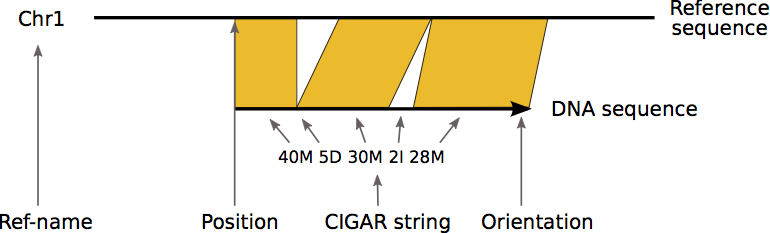
\includegraphics{img/SAM_BAM.png}
\caption{SAM format}
\end{figure}

    \hypertarget{exercises}{%
\subsubsection{Exercises}\label{exercises}}

Let's have a look at example.sam. This file contains only a subset of
the alignment section of a BAM-file that we will look closer at soon.
Notice that we can use the standard UNIX operations like \textbf{cat} on
this file.

    \begin{tcolorbox}[breakable, size=fbox, boxrule=1pt, pad at break*=1mm,colback=cellbackground, colframe=cellborder]
\prompt{In}{incolor}{ }{\boxspacing}
\begin{Verbatim}[commandchars=\\\{\}]
cat data/example.sam
\end{Verbatim}
\end{tcolorbox}

    \textbf{Q8: What is the mapping quality of ERR003762.5016205? (Hint: can
you use grep and awk to find this?)}

    \begin{tcolorbox}[breakable, size=fbox, boxrule=1pt, pad at break*=1mm,colback=cellbackground, colframe=cellborder]
\prompt{In}{incolor}{ }{\boxspacing}
\begin{Verbatim}[commandchars=\\\{\}]

\end{Verbatim}
\end{tcolorbox}

    \textbf{Q9: What is the CIGAR string for ERR003814.6979522? (Hint: we
will go through the meaning of CIGAR strings in the next section)}

    \begin{tcolorbox}[breakable, size=fbox, boxrule=1pt, pad at break*=1mm,colback=cellbackground, colframe=cellborder]
\prompt{In}{incolor}{ }{\boxspacing}
\begin{Verbatim}[commandchars=\\\{\}]

\end{Verbatim}
\end{tcolorbox}

    \textbf{Q10: What is the inferred insert size of ERR003814.1408899?}

    \begin{tcolorbox}[breakable, size=fbox, boxrule=1pt, pad at break*=1mm,colback=cellbackground, colframe=cellborder]
\prompt{In}{incolor}{ }{\boxspacing}
\begin{Verbatim}[commandchars=\\\{\}]

\end{Verbatim}
\end{tcolorbox}

    \hypertarget{cigar-string}{%
\subsubsection{CIGAR string}\label{cigar-string}}

Column 6 of the alignment is the CIGAR string for that alignment. The
CIGAR string provides a compact representation of sequence alignment.
Have a look at the table below. It contains the meaning of all different
symbols of a CIGAR string:

\begin{longtable}[]{@{}ll@{}}
\hline
Symbol & Meaning\tabularnewline
\hline
\endhead
M & alignment match or mismatch\tabularnewline
= & sequence match\tabularnewline
X & sequence mismatch\tabularnewline
I & insertion into the read (sample sequenced)\tabularnewline
D & deletion from the read (sample sequenced)\tabularnewline
S & soft clipping (clipped sequences present in SEQ)\tabularnewline
H & hard clipping (clipped sequences NOT present in SEQ)\tabularnewline
N & skipped region from the reference\tabularnewline
P & padding (silent deletion from padded reference)\tabularnewline
\hline
\end{longtable}

Below are two examples describing the CIGAR string in more detail.

\textbf{Example 1:}\\
Ref:~~~~~ACGTACGTACGTACGT\\
Read:~~ACGT-~-~-~-~ACGTACGA\\
Cigar: 4M 4D 8M

The first four bases in the read are the same as in the reference, so we
can represent these as 4M in the CIGAR string. Next comes 4 deletions,
represented by 4D, followed by 7 alignment matches and one alignment
mismatch, represented by 8M. Note that the mismatch at position 16 is
included in 8M. This is because it still aligns to the reference.

\textbf{Example 2:}\\
Ref:~~~~~ACTCAGTG-~-~GT\\
Read:~~ACGCA-~TGCAGTtagacgt\\
Cigar: 5M 1D 2M 2I 2M 7S

Here we start off with 5 alignment matches and mismatches, followed by
one deletion. Then we have two more alignment matches, two insertions
and two more matches. At the end, we have seven soft clippings, 7S.
These are clipped sequences that are present in the SEQ (Query SEQuence
on the same strand as the reference).

\hypertarget{exercises}{%
\subsubsection{Exercises}\label{exercises}}

\textbf{Q11: What does the CIGAR from Q9 mean?}

    \begin{tcolorbox}[breakable, size=fbox, boxrule=1pt, pad at break*=1mm,colback=cellbackground, colframe=cellborder]
\prompt{In}{incolor}{ }{\boxspacing}
\begin{Verbatim}[commandchars=\\\{\}]

\end{Verbatim}
\end{tcolorbox}

    \textbf{Q12: How would you represent the following alignment with a
CIGAR string?}

Ref:~~~~~ACGT-~-~-~-~ACGTACGT\\
Read:~~ACGTACGTACGTACGT

    \begin{tcolorbox}[breakable, size=fbox, boxrule=1pt, pad at break*=1mm,colback=cellbackground, colframe=cellborder]
\prompt{In}{incolor}{ }{\boxspacing}
\begin{Verbatim}[commandchars=\\\{\}]

\end{Verbatim}
\end{tcolorbox}

    \hypertarget{flags}{%
\subsubsection{Flags}\label{flags}}

Column 2 of the alignment contains a combination of bitwise FLAGs
describing the alignment. The following table contains the information
you can get from the bitwise FLAGs:

\begin{longtable}[]{@{}llll@{}}
\hline
Hex & Dec & Flag & Description\tabularnewline
\hline
\endhead
0x1 & 1 & PAIRED & paired-end (or multiple-segment) sequencing
technology\tabularnewline
0x2 & 2 & PROPER\_PAIR & each segment properly aligned according to the
aligner\tabularnewline
0x4 & 4 & UNMAP & segment unmapped\tabularnewline
0x8 & 8 & MUNMAP & next segment in the template unmapped\tabularnewline
0x10 & 16 & REVERSE & SEQ is reverse complemented\tabularnewline
0x20 & 32 & MREVERSE & SEQ of the next segment in the template is
reversed\tabularnewline
0x40 & 64 & READ1 & the first segment in the template\tabularnewline
0x80 & 128 & READ2 & the last segment in the template\tabularnewline
0x100 & 256 & SECONDARY & secondary alignment\tabularnewline
0x200 & 512 & QCFAIL & not passing quality controls\tabularnewline
0x400 & 1024 & DUP & PCR or optical duplicate\tabularnewline
0x800 & 2048 & SUPPLEMENTARY & supplementary alignment\tabularnewline
\hline
\end{longtable}

For example, if you have an alignment with FLAG set to 113, this can
only be represented by decimal codes \texttt{64\ +\ 32\ +\ 16\ +\ 1}, so
we know that these four flags apply to the alignment and the alignment
is paired-end, reverse complemented, sequence of the next template/mate
of the read is reversed and the read aligned is the first segment in the
template.

\hypertarget{primary-secondary-and-supplementary-alignments}{%
\paragraph{Primary, secondary and supplementary
alignments}\label{primary-secondary-and-supplementary-alignments}}

A read that aligns to a single reference sequence (including insertions,
deletions, skips and clipping but not direction changes), is a
\textbf{linear alignment}. If a read cannot be represented as a linear
alignment, but instead is represented as a group of linear alignments
without large overlaps, it is called a \textbf{chimeric alignment}.
These can for instance be caused by structural variations. Usually, one
of the linear alignments in a chimeric alignment is considered to be the
\textbf{representative} alignment, and the others are called
\textbf{supplementary}.

Sometimes a read maps equally well to more than one spot. In these
cases, one of the possible alignments is marked as the \textbf{primary}
alignment and the rest are marked as \textbf{secondary} alignments.

\hypertarget{bam}{%
\subsection{BAM}\label{bam}}

BAM (Binary Alignment/Map) format, is a compressed binary version of
SAM. This means that, while SAM is human readable, BAM is only readable
for computers. BAM was developed for fast processing and random access.
To achieve this, BGZF (Block GZIP) compression is used for indexing. BAM
files can be viewed using samtools, and will then have the same format
as a SAM file. The key features of BAM are:

\begin{itemize}
\tightlist
\item
  Can store alignments from most mappers
\item
  Supports multiple sequencing technologies
\item
  Supports indexing for quick retrieval/viewing
\item
  Compact size (e.g.~112Gbp Illumina = 116GB disk space)
\item
  Reads can be grouped into logical groups e.g.~lanes, libraries,
  samples
\item
  Widely supported by variant calling packages and viewers
\end{itemize}

    Since BAM is a binary format, we can't use the standard UNIX operations
directly on this file format. \textbf{Samtools} is a set of programs for
interacting with SAM and BAM files. Using the samtools view command,
print the header of the BAM file:

    \begin{tcolorbox}[breakable, size=fbox, boxrule=1pt, pad at break*=1mm,colback=cellbackground, colframe=cellborder]
\prompt{In}{incolor}{ }{\boxspacing}
\begin{Verbatim}[commandchars=\\\{\}]
samtools view \PYZhy{}H data/NA20538.bam
\end{Verbatim}
\end{tcolorbox}

    \hypertarget{exercises}{%
\subsubsection{Exercises}\label{exercises}}

    \textbf{Q13: What version of the human assembly was used to perform the
alignments? (Hint: Can you spot this somewhere in the @SQ records?)}

    \begin{tcolorbox}[breakable, size=fbox, boxrule=1pt, pad at break*=1mm,colback=cellbackground, colframe=cellborder]
\prompt{In}{incolor}{ }{\boxspacing}
\begin{Verbatim}[commandchars=\\\{\}]

\end{Verbatim}
\end{tcolorbox}

    \textbf{Q14: How many lanes are in this BAM file? (Hint: Do you recall
what RG represents?)}

    \begin{tcolorbox}[breakable, size=fbox, boxrule=1pt, pad at break*=1mm,colback=cellbackground, colframe=cellborder]
\prompt{In}{incolor}{ }{\boxspacing}
\begin{Verbatim}[commandchars=\\\{\}]

\end{Verbatim}
\end{tcolorbox}

    \textbf{Q15: What programs were used to create this BAM file? (Hint:
have a look for the program record, @PG)}

    \begin{tcolorbox}[breakable, size=fbox, boxrule=1pt, pad at break*=1mm,colback=cellbackground, colframe=cellborder]
\prompt{In}{incolor}{ }{\boxspacing}
\begin{Verbatim}[commandchars=\\\{\}]

\end{Verbatim}
\end{tcolorbox}

    \textbf{Q16: What version of bwa was used to align the reads? (Hint: is
there anything in the @PG record that looks like it could be a version
tag?)}

    \begin{tcolorbox}[breakable, size=fbox, boxrule=1pt, pad at break*=1mm,colback=cellbackground, colframe=cellborder]
\prompt{In}{incolor}{ }{\boxspacing}
\begin{Verbatim}[commandchars=\\\{\}]

\end{Verbatim}
\end{tcolorbox}

    The output from running samtools view on a BAM file without any options
is a headerless SAM file. This gets printed to STDOUT in the terminal,
so we will want to pipe it to something. Let's have a look at the first
read of the BAM file:

    \begin{tcolorbox}[breakable, size=fbox, boxrule=1pt, pad at break*=1mm,colback=cellbackground, colframe=cellborder]
\prompt{In}{incolor}{ }{\boxspacing}
\begin{Verbatim}[commandchars=\\\{\}]
samtools view data/NA20538.bam \PY{p}{|} head \PYZhy{}n \PY{l+m}{1}
\end{Verbatim}
\end{tcolorbox}

    \textbf{Q17: What is the name of the first read? (Hint: have a look at
the \href{formats.ipynb\#Alignment-Section}{alignment section} if you
can't recall the different fields)}

    \begin{tcolorbox}[breakable, size=fbox, boxrule=1pt, pad at break*=1mm,colback=cellbackground, colframe=cellborder]
\prompt{In}{incolor}{ }{\boxspacing}
\begin{Verbatim}[commandchars=\\\{\}]

\end{Verbatim}
\end{tcolorbox}

    \textbf{Q18: What position does the alignment of the read start at?}

    \begin{tcolorbox}[breakable, size=fbox, boxrule=1pt, pad at break*=1mm,colback=cellbackground, colframe=cellborder]
\prompt{In}{incolor}{ }{\boxspacing}
\begin{Verbatim}[commandchars=\\\{\}]

\end{Verbatim}
\end{tcolorbox}

    \hypertarget{cram}{%
\subsection{CRAM}\label{cram}}

Even though BAM files are compressed, they are still very large.
Typically they use 1.5-2 bytes for each base pair of sequencing data
that they contain, and while disk capacity is ever improving, increases
in disk capacity are being far outstripped by sequencing technologies.

    \begin{figure}[!h]
\centering
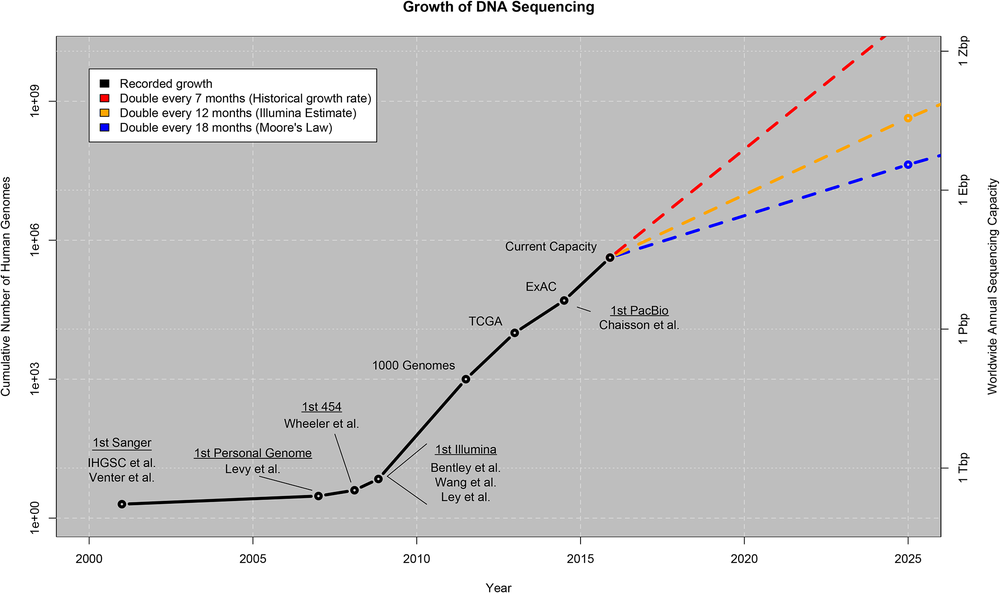
\includegraphics{img/compression_cram.png}
\caption{Growth of DNA sequencing}
\end{figure}

    BAM stores all of the data, this includes every read base, every base
quality, and it uses a single conventional compression technique for all
types of data. CRAM was designed for better compression of genomic data
than SAM/BAM. CRAM uses three important concepts:

\begin{itemize}
\tightlist
\item
  Reference based compression
\item
  Controlled loss of quality information
\item
  Different compression methods to suit the type of data, e.g.~base
  qualities vs.~metadata vs.~extra tags
\end{itemize}

The figure below displays how reference-based compression works. Instead
of saving all the bases of all the reads, only the nucleotides that
differ from the reference, and their positions, are kept.

    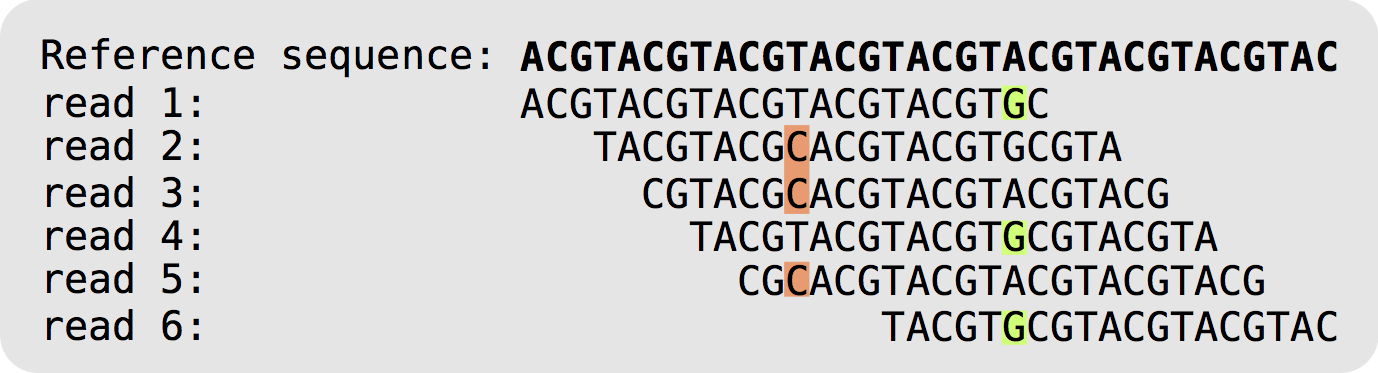
\includegraphics{img/CRAM_format.png}

    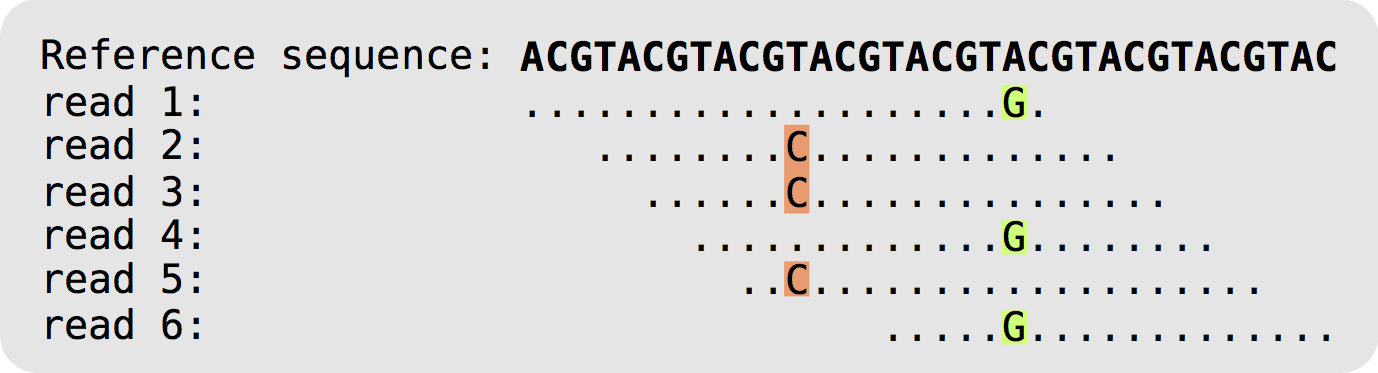
\includegraphics{img/CRAM_format2.png}

    In lossless (no information is lost) mode a CRAM file is 60\% of the
size of a BAM file, so archives and sequencing centres have moved from
BAM to CRAM.

Since samtools 1.3, CRAM files can be read in the same way that BAM
files can. We will look closer at how you can convert between SAM, BAM
and CRAM formats in the next section.

    \hypertarget{indexing}{%
\subsection{Indexing}\label{indexing}}

To allow for fast random access of regions in BAM and CRAM files, they
can be indexed. The files must first be coordinate-sorted rather that
sorted by read name. This can be done using \textbf{samtools sort}. If
no options are supplied, it will by default sort by the left-most
position of the reference.

    \begin{tcolorbox}[breakable, size=fbox, boxrule=1pt, pad at break*=1mm,colback=cellbackground, colframe=cellborder]
\prompt{In}{incolor}{ }{\boxspacing}
\begin{Verbatim}[commandchars=\\\{\}]
samtools sort \PYZhy{}o data/NA20538\PYZus{}sorted.bam data/NA20538.bam
\end{Verbatim}
\end{tcolorbox}

    Now we can use \textbf{samtools index} to create an index file (.bai)
for our sorted BAM file:

    \begin{tcolorbox}[breakable, size=fbox, boxrule=1pt, pad at break*=1mm,colback=cellbackground, colframe=cellborder]
\prompt{In}{incolor}{ }{\boxspacing}
\begin{Verbatim}[commandchars=\\\{\}]
samtools index data/NA20538\PYZus{}sorted.bam
\end{Verbatim}
\end{tcolorbox}

    To look for reads mapped to a specific region, we can use
\textbf{samtools view} and specify the region we are interested in as:
RNAME{[}:STARTPOS{[}-ENDPOS{]}{]}. For example, if we wanted to look at
all the reads mapped to a region called chr4, we could use:

    \texttt{samtools\ view\ alignment.bam\ chr4}

    To look at the region on chr4 beginning at position 1,000,000 and ending
at the end of the chromosome, we can do:

    \texttt{samtools\ view\ alignment.bam\ chr4:1000000}

    And to explore the 1001bp long region on chr4 beginning at position
1,000 and ending at position 2,000, we can use:

    \texttt{samtools\ view\ alignment.bam\ chr4:1000-2000}

    \hypertarget{exercises}{%
\subsubsection{Exercises}\label{exercises}}

\textbf{Q19: How many reads are mapped to region 20025000-20030000 on
chromosome 1?}

    \begin{tcolorbox}[breakable, size=fbox, boxrule=1pt, pad at break*=1mm,colback=cellbackground, colframe=cellborder]
\prompt{In}{incolor}{ }{\boxspacing}
\begin{Verbatim}[commandchars=\\\{\}]

\end{Verbatim}
\end{tcolorbox}

    \hypertarget{vcf}{%
\subsection{VCF}\label{vcf}}

The VCF file format was introduced to store variation data. VCF consists
of tab-delimited text and is parsable by standard UNIX commands which
makes it flexible and user-extensible. The figure below provides an
overview of the different components of a VCF file:

    \begin{figure}[!h]
\centering
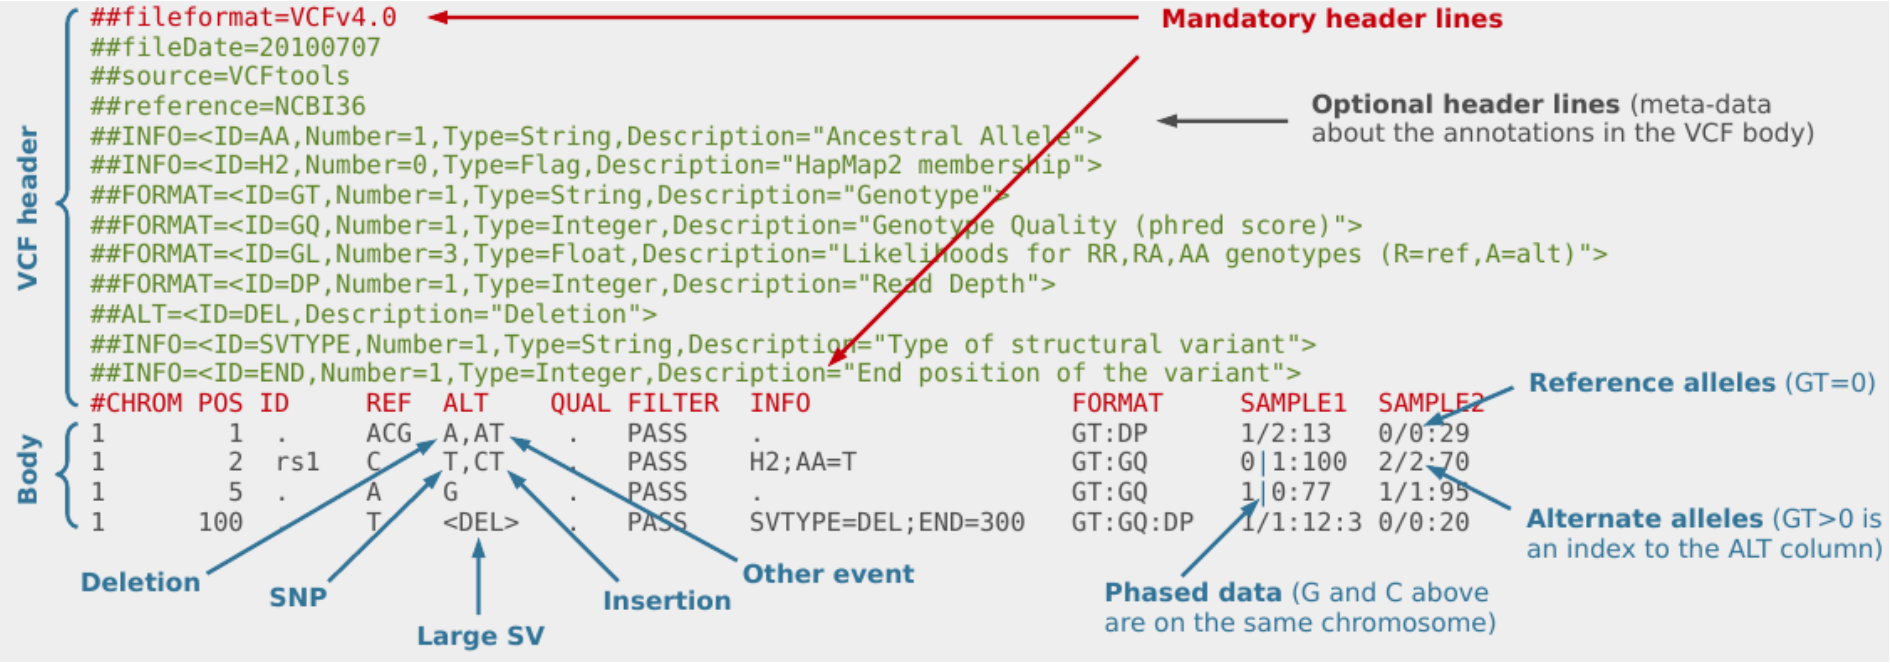
\includegraphics{img/VCF1.png}
\caption{VCF format}
\end{figure}

    \hypertarget{vcf-header}{%
\subsubsection{VCF header}\label{vcf-header}}

The VCF header consists of meta-information lines (starting with
\texttt{\#\#}) and a header line (starting with \texttt{\#}). All
meta-information lines are optional and can be put in any order, except
for \textit{fileformat}. This holds the information about which version of
VCF is used and must come first.

The meta-information lines consist of key=value pairs. Examples of
meta-information lines that can be included are \#\#INFO, \#\#FORMAT and
\#\#reference. The values can consist of multiple fields enclosed by
\texttt{\textless{}\textgreater{}}. More information about these fields
is available in the VCF specification
\url{http://samtools.github.io/hts-specs/VCFv4.3.pdf}. This can be
accessed using a web browser and there is a copy in the QC directory.

\hypertarget{header-line}{%
\paragraph{Header line}\label{header-line}}

The header line starts with \texttt{\#} and consists of 8 required
fields:

\begin{enumerate}
\def\labelenumi{\arabic{enumi}.}
\tightlist
\item
  CHROM: an identifier from the reference genome
\item
  POS: the reference position
\item
  ID: a list of unique identifiers (where available)
\item
  REF: the reference base(s)
\item
  ALT: the alternate base(s)
\item
  QUAL: a phred-scaled quality score
\item
  FILTER: filter status
\item
  INFO: additional information
\end{enumerate}

If the file contains genotype data, the required fields are also
followed by a FORMAT column header, and then a number of sample IDs. The
FORMAT field specifies the data types and order. Some examples of these
data types are:

\begin{itemize}
\tightlist
\item
  GT: Genotype, encoded as allele values separated by either / or
  \textbar{}
\item
  DP: Read depth at this position for this sample
\item
  GQ: Conditional genotype quality, encoded as a phred quality
\end{itemize}

\hypertarget{body}{%
\subsubsection{Body}\label{body}}

In the body of the VCF, each row contains information about a position
in the genome along with genotype information on samples for each
position, all according to the fields in the header line.

\hypertarget{bcf}{%
\subsection{BCF}\label{bcf}}

BCF is a compressed binary representation of VCF.

VCF can be compressed with BGZF (bgzip) and indexed with TBI or CSI
(tabix), but even compressed it can still be very big. For example, a
compressed VCF with 3781 samples of human data will be 54 GB for
chromosome 1, and 680 GB for the whole genome. VCFs can also be slow to
parse, as text conversion is slow. The main bottleneck is the ``FORMAT''
fields. For this reason the BCF format was developed.

In BCF files the fields are rearranged for fast access. The following
images show the process of converting a VCF file into a BCF file.

    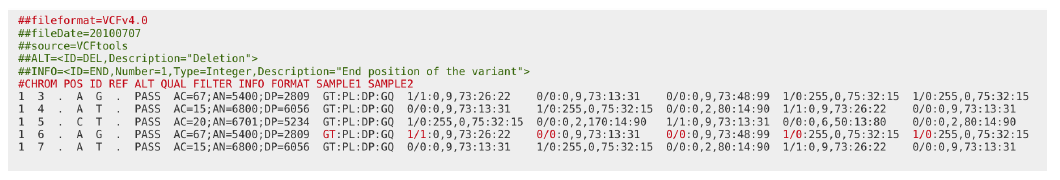
\includegraphics{img/VCF2.png}

    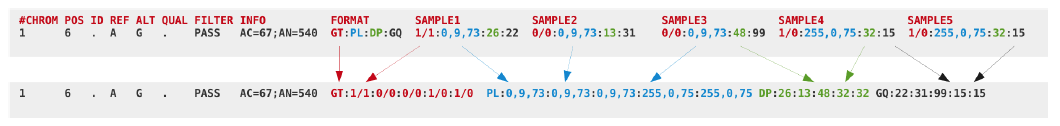
\includegraphics{img/VCF3.png}

    Bcftools comprises a set of programs for interacting with VCF and BCF
files. It can be used to convert between VCF and BCF and to view or
extract records from a region.

\hypertarget{bcftools-view}{%
\subsubsection{bcftools view}\label{bcftools-view}}

Let's have a look at the header of the file 1kg.bcf in the data
directory. Note that bcftools uses \textbf{\texttt{-h}} to print only
the header, while samtools uses \textbf{\texttt{-H}} for this.

    \begin{tcolorbox}[breakable, size=fbox, boxrule=1pt, pad at break*=1mm,colback=cellbackground, colframe=cellborder]
\prompt{In}{incolor}{ }{\boxspacing}
\begin{Verbatim}[commandchars=\\\{\}]
bcftools view \PYZhy{}h data/1kg.bcf
\end{Verbatim}
\end{tcolorbox}

    Similarly to BAM, BCF supports random access, that is, fast retrieval
from a given region. For this, the file must be indexed:

    \begin{tcolorbox}[breakable, size=fbox, boxrule=1pt, pad at break*=1mm,colback=cellbackground, colframe=cellborder]
\prompt{In}{incolor}{ }{\boxspacing}
\begin{Verbatim}[commandchars=\\\{\}]
bcftools index data/1kg.bcf
\end{Verbatim}
\end{tcolorbox}

    Now we can extract all records from the region 20:24042765-24043073,
using the \textbf{\texttt{-r}} option. The \textbf{\texttt{-H}} option
will make sure we don't include the header in the output:

    \begin{tcolorbox}[breakable, size=fbox, boxrule=1pt, pad at break*=1mm,colback=cellbackground, colframe=cellborder]
\prompt{In}{incolor}{ }{\boxspacing}
\begin{Verbatim}[commandchars=\\\{\}]
bcftools view \PYZhy{}H \PYZhy{}r \PY{l+m}{20}:24042765\PYZhy{}24043073 data/1kg.bcf
\end{Verbatim}
\end{tcolorbox}

    \hypertarget{bcftools-query}{%
\subsubsection{bcftools query}\label{bcftools-query}}

The versatile \textbf{bcftools query} command can be used to extract any
VCF field. Combined with standard UNIX commands, this gives a powerful
tool for quick querying of VCFs. Have a look at the usage options:

    \begin{tcolorbox}[breakable, size=fbox, boxrule=1pt, pad at break*=1mm,colback=cellbackground, colframe=cellborder]
\prompt{In}{incolor}{ }{\boxspacing}
\begin{Verbatim}[commandchars=\\\{\}]
bcftools query \PYZhy{}h
\end{Verbatim}
\end{tcolorbox}

    Let's try out some useful options. As you can see from the usage,
\textbf{\texttt{-l}} will print a list of all the samples in the file.
Give this a go:

    \begin{tcolorbox}[breakable, size=fbox, boxrule=1pt, pad at break*=1mm,colback=cellbackground, colframe=cellborder]
\prompt{In}{incolor}{ }{\boxspacing}
\begin{Verbatim}[commandchars=\\\{\}]
bcftools query \PYZhy{}l data/1kg.bcf
\end{Verbatim}
\end{tcolorbox}

    Another very useful option is \textbf{\texttt{-s}} which allows you to
extract all the data relating to a particular sample. This is a
\href{http://samtools.github.io/bcftools/bcftools.html\#common_options}{common
option} meaning it can be used for many bcftools commands, like
\texttt{bcftools\ view}. Try this for sample HG00131:

    \begin{tcolorbox}[breakable, size=fbox, boxrule=1pt, pad at break*=1mm,colback=cellbackground, colframe=cellborder]
\prompt{In}{incolor}{ }{\boxspacing}
\begin{Verbatim}[commandchars=\\\{\}]
bcftools view \PYZhy{}s HG00131 data/1kg.bcf \PY{p}{|} head \PYZhy{}n \PY{l+m}{50}
\end{Verbatim}
\end{tcolorbox}

    The format option, \textbf{\texttt{-f}} can be used to select what gets
printed from your query command. For example, the following will print
the position, reference base and alternate base for sample HG00131,
separated by tabs:

    \begin{tcolorbox}[breakable, size=fbox, boxrule=1pt, pad at break*=1mm,colback=cellbackground, colframe=cellborder]
\prompt{In}{incolor}{ }{\boxspacing}
\begin{Verbatim}[commandchars=\\\{\}]
bcftools query \PYZhy{}f\PY{l+s+s1}{\PYZsq{}\PYZpc{}POS\PYZbs{}t\PYZpc{}REF\PYZbs{}t\PYZpc{}ALT\PYZbs{}n\PYZsq{}} \PYZhy{}s HG00131 data/1kg.bcf \PY{p}{|} head
\end{Verbatim}
\end{tcolorbox}

    Finally, let's look at the \textbf{\texttt{-i}} option. With this option
we can select only sites for which a particular expression is true. For
instance, if we only want to look at sites that have at least 2
alternate alleles, we can use the following expression (piped to
\texttt{head} to only show a subset of the output):

    \begin{tcolorbox}[breakable, size=fbox, boxrule=1pt, pad at break*=1mm,colback=cellbackground, colframe=cellborder]
\prompt{In}{incolor}{ }{\boxspacing}
\begin{Verbatim}[commandchars=\\\{\}]
bcftools query \PYZhy{}f\PY{l+s+s1}{\PYZsq{}\PYZpc{}CHROM\PYZbs{}t\PYZpc{}POS\PYZbs{}n\PYZsq{}} \PYZhy{}i \PY{l+s+s1}{\PYZsq{}AC[0]\PYZgt{}2\PYZsq{}} data/1kg.bcf \PY{p}{|} head
\end{Verbatim}
\end{tcolorbox}

    We use \textbf{\texttt{-i}} with the expression
\texttt{AC{[}0{]}\textgreater{}2}. AC is an info field that holds the
\_\_a\_\_llele \_\_c\_\_ount. Some fields can hold multiple values, so
we use \texttt{AC{[}0{]}\textgreater{}2} to indicate that we are looking
for the first value (this is zero indexed, and hence starts at 0 instead
of 1), and that this value should be \textgreater{} 2. To format our
output, we use \textbf{\texttt{-f}} to specify that we want to print the
chromosome name and position.

There is more information about expressions on the bcftools manual page
\url{http://samtools.github.io/bcftools/bcftools.html\#expressions}

    \hypertarget{exercises}{%
\subsubsection{Exercises}\label{exercises}}

Now, try and answer the following questions about the file 1kg.bcf in
the data directory. For more information about the different usage
options you can open the bcftools query manual page
\url{http://samtools.github.io/bcftools/bcftools.html\#query} in a web
browser.

    \textbf{Q20: What version of the human assembly do the coordinates refer
to?}

    \begin{tcolorbox}[breakable, size=fbox, boxrule=1pt, pad at break*=1mm,colback=cellbackground, colframe=cellborder]
\prompt{In}{incolor}{ }{\boxspacing}
\begin{Verbatim}[commandchars=\\\{\}]

\end{Verbatim}
\end{tcolorbox}

    \textbf{Q21: How many samples are there in the BCF?}

    \begin{tcolorbox}[breakable, size=fbox, boxrule=1pt, pad at break*=1mm,colback=cellbackground, colframe=cellborder]
\prompt{In}{incolor}{ }{\boxspacing}
\begin{Verbatim}[commandchars=\\\{\}]

\end{Verbatim}
\end{tcolorbox}

    \textbf{Q22: What is the genotype of the sample HG00107 at the position
20:24019472? (Hint: use the combination of -r, -s, and -f options)}

    \begin{tcolorbox}[breakable, size=fbox, boxrule=1pt, pad at break*=1mm,colback=cellbackground, colframe=cellborder]
\prompt{In}{incolor}{ }{\boxspacing}
\begin{Verbatim}[commandchars=\\\{\}]

\end{Verbatim}
\end{tcolorbox}

    \textbf{Q23: How many positions are there with more than 10 alternate
alleles? (Hint: use the -i filtering option)}

    \begin{tcolorbox}[breakable, size=fbox, boxrule=1pt, pad at break*=1mm,colback=cellbackground, colframe=cellborder]
\prompt{In}{incolor}{ }{\boxspacing}
\begin{Verbatim}[commandchars=\\\{\}]

\end{Verbatim}
\end{tcolorbox}

    \textbf{Q24: In how many positions does HG00107 have a non-reference
genotype and a read depth bigger than 10? (Hint: you can use pipes to
combine bcftools queries)}

    \begin{tcolorbox}[breakable, size=fbox, boxrule=1pt, pad at break*=1mm,colback=cellbackground, colframe=cellborder]
\prompt{In}{incolor}{ }{\boxspacing}
\begin{Verbatim}[commandchars=\\\{\}]

\end{Verbatim}
\end{tcolorbox}

    \hypertarget{gvcf}{%
\subsection{gVCF}\label{gvcf}}

Often it is not enough to know variant sites only. For instance, we
don't know if a site was dropped because it matches the reference or
because the data is missing. We sometimes need evidence for both variant
and non-variant positions in the genome. In gVCF format, blocks of
reference-only sites can be represented in a single record using the
``INFO/END'' tag. Symbolic alleles (\textless*\textgreater) are used for
incremental calling:

    \begin{figure}[!h]
\centering
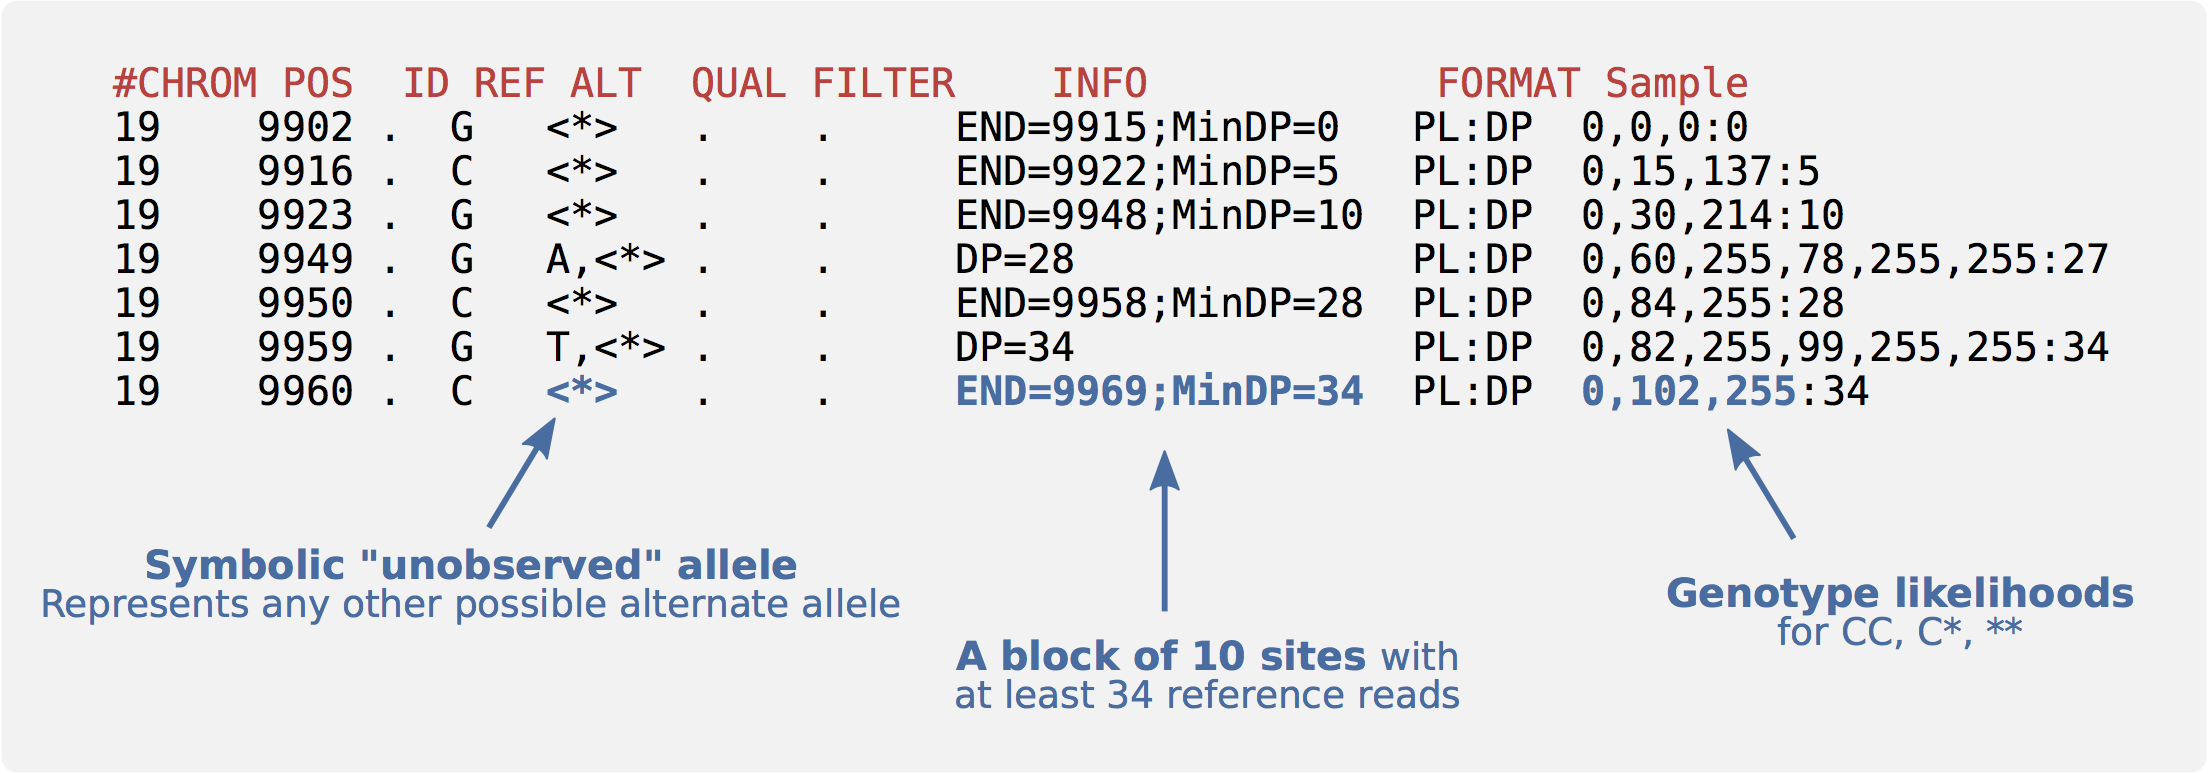
\includegraphics{img/gVCF.png}
\caption{gVCF}
\end{figure}

    \hypertarget{exercises}{%
\subsubsection{Exercises}\label{exercises}}

\textbf{Q25: In the above example, what is the size of the
reference-only block starting at position 9923?}

    \begin{tcolorbox}[breakable, size=fbox, boxrule=1pt, pad at break*=1mm,colback=cellbackground, colframe=cellborder]
\prompt{In}{incolor}{ }{\boxspacing}
\begin{Verbatim}[commandchars=\\\{\}]

\end{Verbatim}
\end{tcolorbox}

    \textbf{Q26: For the same block, what is the first base?}

    \begin{tcolorbox}[breakable, size=fbox, boxrule=1pt, pad at break*=1mm,colback=cellbackground, colframe=cellborder]
\prompt{In}{incolor}{ }{\boxspacing}
\begin{Verbatim}[commandchars=\\\{\}]

\end{Verbatim}
\end{tcolorbox}

    \textbf{Q27: How many reference reads does the block have?}

    \begin{tcolorbox}[breakable, size=fbox, boxrule=1pt, pad at break*=1mm,colback=cellbackground, colframe=cellborder]
\prompt{In}{incolor}{ }{\boxspacing}
\begin{Verbatim}[commandchars=\\\{\}]

\end{Verbatim}
\end{tcolorbox}

    Now continue to the next section of the tutorial:
\href{conversion.ipynb}{File conversion}.


    % Add a bibliography block to the postdoc



\newpage





    \hypertarget{file-conversion}{%
\section{File conversion}\label{file-conversion}}

In this section we are going to look at how to convert from one file
format to another. There are many tools available for converting between
file formats, and we will use some of the most common ones: samtools,
bcftools and Picard.

\hypertarget{sam-to-bam}{%
\subsection{SAM to BAM}\label{sam-to-bam}}

To convert from SAM to BAM format we are going to use the
\textbf{\texttt{samtools\ view}} command. In this instance, we would
like to include the SAM header, so we use the \textbf{\texttt{-h}}
option:

    \begin{tcolorbox}[breakable, size=fbox, boxrule=1pt, pad at break*=1mm,colback=cellbackground, colframe=cellborder]
\prompt{In}{incolor}{ }{\boxspacing}
\begin{Verbatim}[commandchars=\\\{\}]
samtools view \PYZhy{}h data/NA20538.bam \PYZgt{} data/NA20538.sam
\end{Verbatim}
\end{tcolorbox}

    Now, have a look at the first ten lines of the SAM file. They should
look like they did in the previous section when you viewed the BAM file
header.

    \begin{tcolorbox}[breakable, size=fbox, boxrule=1pt, pad at break*=1mm,colback=cellbackground, colframe=cellborder]
\prompt{In}{incolor}{ }{\boxspacing}
\begin{Verbatim}[commandchars=\\\{\}]
head data/NA20538.sam
\end{Verbatim}
\end{tcolorbox}

    Well that was easy! And converting SAM to BAM is just as
straightforward. This time there is no need for the \texttt{-h} option,
however we have to tell samtools that we want the output in BAM format.
We do so by adding the \textbf{\texttt{-b}} option:

    \begin{tcolorbox}[breakable, size=fbox, boxrule=1pt, pad at break*=1mm,colback=cellbackground, colframe=cellborder]
\prompt{In}{incolor}{ }{\boxspacing}
\begin{Verbatim}[commandchars=\\\{\}]
samtools view \PYZhy{}b data/NA20538.sam \PYZgt{} data/NA20538\PYZus{}2.bam
\end{Verbatim}
\end{tcolorbox}

    Samtools is very well documented, so for more usage options and
functions, have a look at the samtools manual
\url{http://www.htslib.org/doc/samtools-1.0.html}.

    \hypertarget{bam-to-cram}{%
\subsection{BAM to CRAM}\label{bam-to-cram}}

From samtools version 1.3, support for CRAM format was introduced. This
means that the samtools view command can also be used to convert a BAM
file to CRAM format. In the data directory there is a BAM file called
yeast.bam that was created from S. cerevisiae Illumina sequencing data.
There is also a reference genome in the directory, called
Saccharomyces\_cerevisiae.EF4.68.dna.toplevel.fa. For the conversion, an
index file (.fai) for the reference must be created. This can be done
using \textbf{\texttt{samtools\ faidx}}. However, as we will see,
samtools will generate this file on the fly when we specify a reference
file using the \texttt{-F} option.

To convert to CRAM, we use the \textbf{\texttt{-C}} option to tell
samtools we want the output as CRAM, and the \textbf{\texttt{-T}} option
to specify what reference file to use for the conversion. We also use
the \textbf{\texttt{-o}} option to specify the name of the output file.
Give this a go:

    \begin{tcolorbox}[breakable, size=fbox, boxrule=1pt, pad at break*=1mm,colback=cellbackground, colframe=cellborder]
\prompt{In}{incolor}{ }{\boxspacing}
\begin{Verbatim}[commandchars=\\\{\}]
samtools view \PYZhy{}C \PY{l+s+se}{\PYZbs{}}
    \PYZhy{}T data/Saccharomyces\PYZus{}cerevisiae.EF4.68.dna.toplevel.fa \PY{l+s+se}{\PYZbs{}}
    \PYZhy{}o data/yeast.cram data/yeast.bam
\end{Verbatim}
\end{tcolorbox}

    Have a look at what files were created:

    \begin{tcolorbox}[breakable, size=fbox, boxrule=1pt, pad at break*=1mm,colback=cellbackground, colframe=cellborder]
\prompt{In}{incolor}{ }{\boxspacing}
\begin{Verbatim}[commandchars=\\\{\}]
ls \PYZhy{}l data
\end{Verbatim}
\end{tcolorbox}

    As you can see, this has created an index file for the reference genome
called Saccharomyces\_cerevisiae.EF4.68.dna.toplevel.fa.fai and the CRAM
file yeast.cram.

    \hypertarget{exercises}{%
\subsubsection{Exercises}\label{exercises}}

\textbf{Q1: Since CRAM files use reference-based compression, we expect
the CRAM file to be smaller than the BAM file. What is the size of the
CRAM file?}

    \begin{tcolorbox}[breakable, size=fbox, boxrule=1pt, pad at break*=1mm,colback=cellbackground, colframe=cellborder]
\prompt{In}{incolor}{ }{\boxspacing}
\begin{Verbatim}[commandchars=\\\{\}]

\end{Verbatim}
\end{tcolorbox}

    \textbf{Q2: Is your CRAM file smaller than the original BAM file?}

    \begin{tcolorbox}[breakable, size=fbox, boxrule=1pt, pad at break*=1mm,colback=cellbackground, colframe=cellborder]
\prompt{In}{incolor}{ }{\boxspacing}
\begin{Verbatim}[commandchars=\\\{\}]

\end{Verbatim}
\end{tcolorbox}

    To convert CRAM back to BAM, simply change \texttt{-C} to \texttt{-b}
and change places for the input and output CRAM/BAM:

\begin{verbatim}
samtools view -b -T data/Saccharomyces_cerevisiae.EF4.68.dna.toplevel.fa \
    -o data/yeast.bam data/yeast.cram
\end{verbatim}

    \hypertarget{fastq-to-sam}{%
\subsection{FASTQ to SAM}\label{fastq-to-sam}}

As mentioned in the previous section of this tutorial, SAM format is
mainly used to store alignment data. However, in some cases we may want
to store unaligned data in SAM format and for this we can use the picard
tools \textbf{\texttt{FastqToSam}} application. Picard tools is a Java
application that comes with a number of useful options for manipulating
high-throughput sequencing data. Apart from FASTQ to SAM, we won't go
into any detail about Picard tools in this tutorial, but feel free to
explore it on the \href{https://broadinstitute.github.io/picard/}{Picard
tools website}. To convert the FASTQ files of lane 13681\_1\#18 to
unaligned SAM format, run:

    \begin{tcolorbox}[breakable, size=fbox, boxrule=1pt, pad at break*=1mm,colback=cellbackground, colframe=cellborder]
\prompt{In}{incolor}{ }{\boxspacing}
\begin{Verbatim}[commandchars=\\\{\}]
PicardCommandLine FastqToSam \PY{n+nv}{F1}\PY{o}{=}data/13681\PYZus{}1\PYZsh{}18\PYZus{}1.fastq.gz \PY{l+s+se}{\PYZbs{}}
    \PY{n+nv}{F2}\PY{o}{=}data/13681\PYZus{}1\PYZsh{}18\PYZus{}2.fastq.gz \PY{l+s+se}{\PYZbs{}}
    \PY{n+nv}{O}\PY{o}{=}data/13681\PYZus{}1\PYZsh{}18.sam \PY{n+nv}{SM}\PY{o}{=}13681\PYZus{}1\PYZsh{}18
\end{Verbatim}
\end{tcolorbox}

    From here you can go on and convert the SAM file to BAM and CRAM, as
described previously. There are also multiple options for specifying
what metadata to include in the SAM header. To see all available
options, run:

    \begin{tcolorbox}[breakable, size=fbox, boxrule=1pt, pad at break*=1mm,colback=cellbackground, colframe=cellborder]
\prompt{In}{incolor}{ }{\boxspacing}
\begin{Verbatim}[commandchars=\\\{\}]
PicardCommandLine FastqToSam \PYZhy{}h
\end{Verbatim}
\end{tcolorbox}

    \hypertarget{cram-to-fastq}{%
\subsection{CRAM to FASTQ}\label{cram-to-fastq}}

Although it is possible to convert CRAM to FASTQ directly using the
\texttt{samtools\ fastq} command, for many applications we need the
fastq files to be ordered so that the order of the reads in the first
file match the order of the reads in the mate file. For this reason, we
will first use \texttt{samtools\ collate} to produce a collated BAM
file. The reference file and its index file that was created when we
converted BAM to CRAM is required for this as well.

    \begin{tcolorbox}[breakable, size=fbox, boxrule=1pt, pad at break*=1mm,colback=cellbackground, colframe=cellborder]
\prompt{In}{incolor}{ }{\boxspacing}
\begin{Verbatim}[commandchars=\\\{\}]
samtools collate data/yeast.cram data/yeast.collated
\end{Verbatim}
\end{tcolorbox}

    The newly produced BAM file will be called yeast.collated.bam. Let's use
this to create two FASTQ files, one for the forward reads and one for
the reverse reads:

    \begin{tcolorbox}[breakable, size=fbox, boxrule=1pt, pad at break*=1mm,colback=cellbackground, colframe=cellborder]
\prompt{In}{incolor}{ }{\boxspacing}
\begin{Verbatim}[commandchars=\\\{\}]
samtools fastq \PYZhy{}1 data/yeast.collated\PYZus{}1.fastq \PY{l+s+se}{\PYZbs{}}
    \PYZhy{}2 data/yeast.collated\PYZus{}2.fastq data/yeast.collated.bam
\end{Verbatim}
\end{tcolorbox}

    For further information and usage options, have a look at the samtools
manual page
\href{http://www.htslib.org/doc/samtools.html}{(http://www.htslib.org/doc/samtools.html)}.

    \hypertarget{vcf-to-bcf}{%
\subsection{VCF to BCF}\label{vcf-to-bcf}}

As we saw in the previous section, bcftools comprises a set of programs
for interacting with VCF/BCF files. In a similar way that samtools view
can be used to convert between SAM, BAM and CRAM,
\textbf{\texttt{bcftools\ view}} can be used to convert between VCF and
BCF. To convert the file called 1kg.bcf to a compressed VCF file called
1kg.vcf.gz, run:

    \begin{tcolorbox}[breakable, size=fbox, boxrule=1pt, pad at break*=1mm,colback=cellbackground, colframe=cellborder]
\prompt{In}{incolor}{ }{\boxspacing}
\begin{Verbatim}[commandchars=\\\{\}]
bcftools view \PYZhy{}O z \PYZhy{}o data/1kg.vcf.gz data/1kg.bcf
\end{Verbatim}
\end{tcolorbox}

    The \textbf{\texttt{-O}} option allows us to specify in what format we
want the output, compressed BCF (b), uncompressed BCF (u), compressed
VCF (z) or uncompressed VCF (v). With the \textbf{\texttt{-o}} option we
can select the name of the output file.

Have a look at what files were generated (the options \texttt{-lrt} will
list the files in reverse chronological order):

    \begin{tcolorbox}[breakable, size=fbox, boxrule=1pt, pad at break*=1mm,colback=cellbackground, colframe=cellborder]
\prompt{In}{incolor}{ }{\boxspacing}
\begin{Verbatim}[commandchars=\\\{\}]
ls \PYZhy{}lrt data
\end{Verbatim}
\end{tcolorbox}

    As you can see, this also generated an index file, 1kg.bcf.csi.

    To convert a VCF file to BCF, we can run a similar command. If we want
to keep the original BCF, we need to give the new one a different name
so that the old one is not overwritten:

    \begin{tcolorbox}[breakable, size=fbox, boxrule=1pt, pad at break*=1mm,colback=cellbackground, colframe=cellborder]
\prompt{In}{incolor}{ }{\boxspacing}
\begin{Verbatim}[commandchars=\\\{\}]
bcftools view \PYZhy{}O b \PYZhy{}o data/1kg\PYZus{}2.bcf data/1kg.vcf.gz
\end{Verbatim}
\end{tcolorbox}

    Now continue to the next section of the tutorial:
\href{assessment.ipynb}{QC assessment of NGS data}.


    % Add a bibliography block to the postdoc



\newpage





    \hypertarget{qc-assessment-of-ngs-data}{%
\section{QC assessment of NGS data}\label{qc-assessment-of-ngs-data}}

QC is an important part of any analysis. In this section we are going to
look at some of the metrics and graphs that can be used to assess the QC
of NGS data.

\hypertarget{base-quality}{%
\subsection{Base quality}\label{base-quality}}

\href{https://en.wikipedia.org/wiki/Illumina_dye_sequencing}{Illumina
sequencing} technology relies on sequencing by synthesis. One of the
most common problems with this is \textbf{dephasing}. For each
sequencing cycle, there is a possibility that the replication machinery
slips and either incorporates more than one nucleotide or perhaps misses
to incorporate one at all. The more cycles that are run (i.e.~the longer
the read length gets), the greater the accumulation of these types of
errors gets. This leads to a heterogeneous population in the cluster,
and a decreased signal purity, which in turn reduces the precision of
the base calling. The figure below shows an example of this.

    \begin{figure}[!h]
\centering
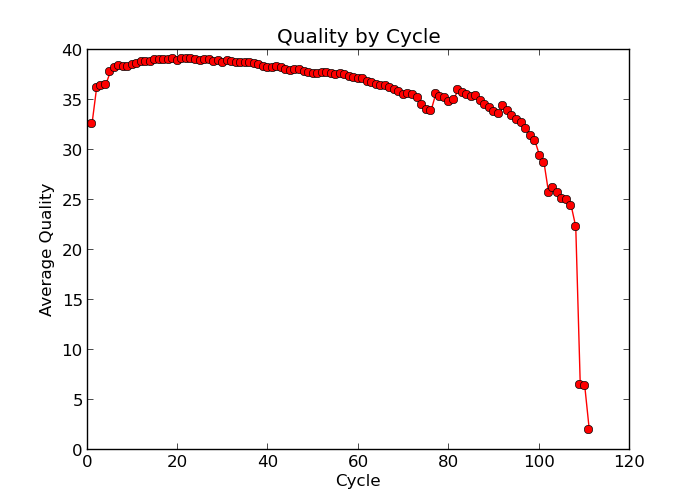
\includegraphics{img/base_qual.png}
\caption{Mean Base Quality}
\end{figure}

    Because of dephasing, it is possible to have high-quality data at the
beginning of the read but really low-quality data towards the end of the
read. In those cases you can decide to trim off the low-quality reads,
for example using a tool called
\href{http://www.usadellab.org/cms/?page=trimmomatic}{Trimmomatic}.

The figures below shows an example of a good sequencing run (left) and a
poor sequencing run (right).

    \begin{figure}[!h]
\centering
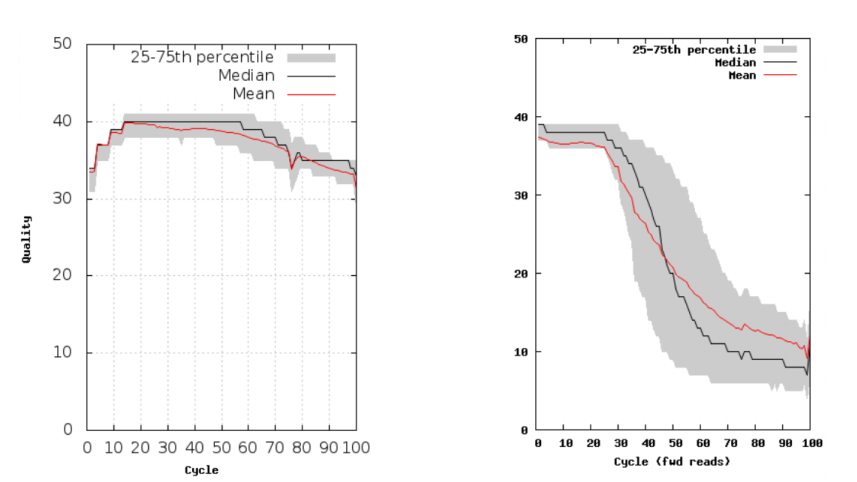
\includegraphics{img/base_qual_comparison.png}
\caption{Base quality}
\end{figure}


    \hypertarget{other-base-calling-errors}{%
\subsection{Other base calling errors}\label{other-base-calling-errors}}

There are several different reasons for a base to be called incorrectly,
as shown in the figure below. \textbf{Phasing noise} and \textbf{signal
decay} is a result of the dephasing issue described above. During
library preparation, \textbf{mixed clusters} can occur if multiple
templates get co-located. These clusters should be removed from the
downstream analysis. \textbf{Boundary effects} occur due to optical
effects when the intensity is uneven across each tile, resulting in
higher intensity found toward the center. \textbf{Cross-talk} occurs
because the emission frequency spectra for each of the four base dyes
partly overlap, creating uncertainty. Finally, for previous sequencing
cycle methods \textbf{T fluorophore accumulation} was an issue, where
incomplete removal of the dye coupled to thymine lead to an ambient
accumulation the nucleotides, causing a false high Thymine trend.

\pagebreak 

    \begin{figure}[!h]
\centering
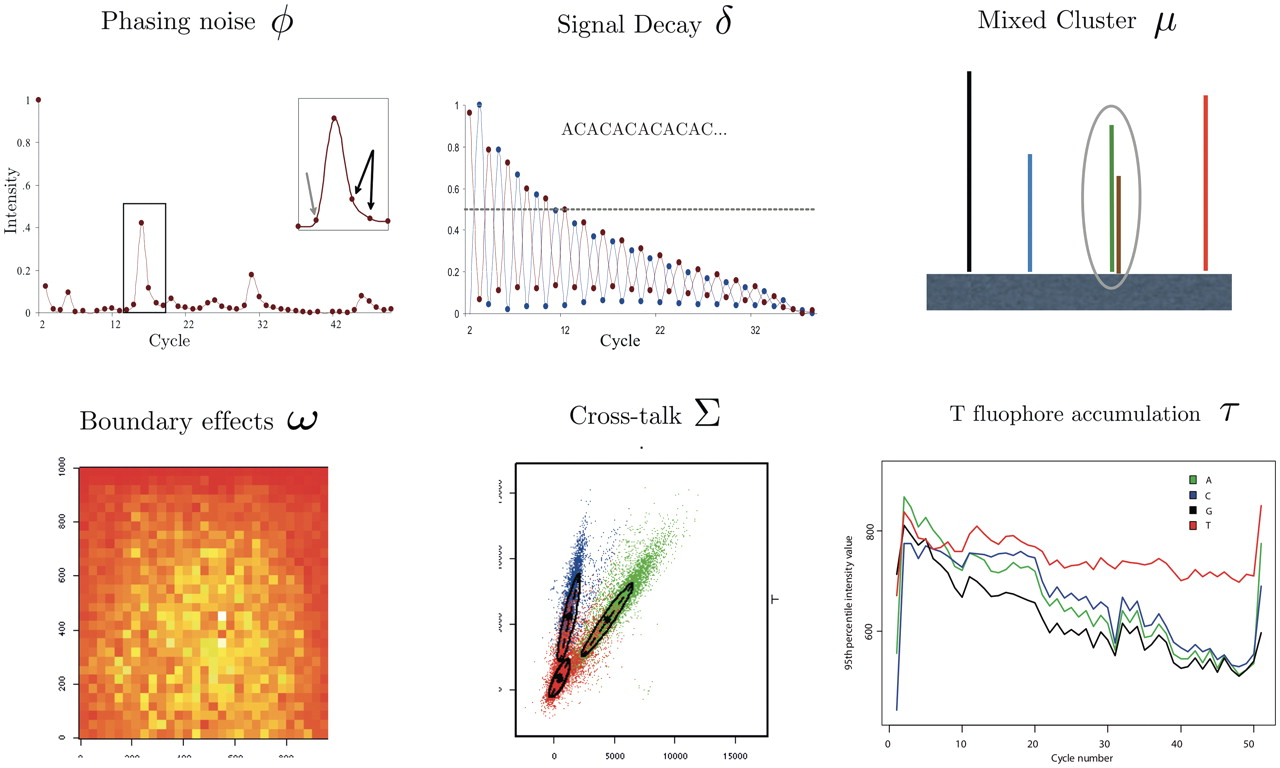
\includegraphics{img/base_calling_errors.jpg}
\caption{Base Calling Errors}
\end{figure}

    \textit{Base-calling for next-generation sequencing platforms}, doi:
\href{https://academic.oup.com/bib/article/12/5/489/268399}{10.1093/bib/bbq077}

\hypertarget{mismatches-per-cycle}{%
\subsection{Mismatches per cycle}\label{mismatches-per-cycle}}

Aligning reads to a high-quality reference genome can provide insight to
the quality of a sequencing run by showing you the mismatches to the
reference sequence. This can help you detect cycle-specific errors.
Mismatches can occur due to two main causes, sequencing errors and
differences between your sample and the reference genome, which is
important to bear in mind when interpreting mismatch graphs. The figure
below shows an example of a good run (left) and a bad one (right). In
the graph on the left, the distribution of the number of mismatches is
even between the cycles, which is what we would expect from a good run.
However, in the graph on the right, two cycles stand out with a lot of
mismatches compared to the other cycles.

    \begin{figure}[!h]
\centering
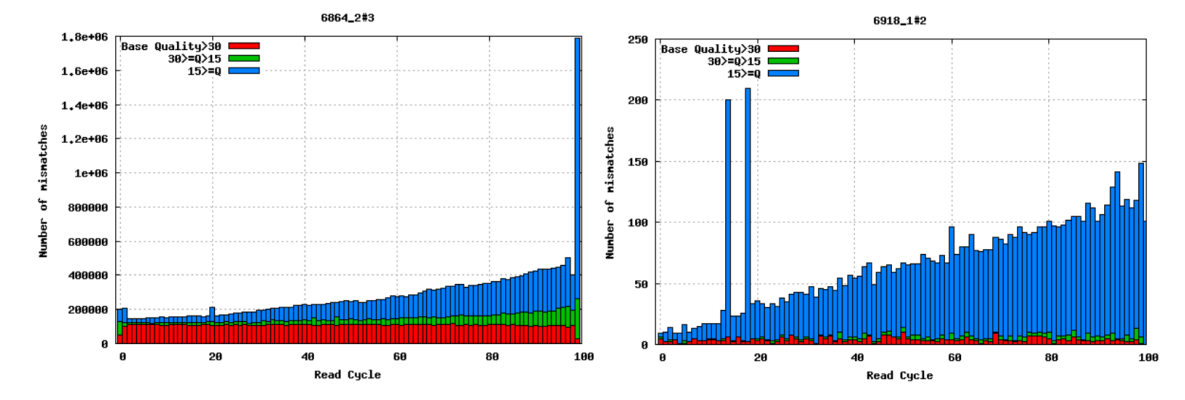
\includegraphics{img/mismatch_per_cycle_comparison.png}
\caption{Mismatches per cycle}
\end{figure}

\pagebreak

    \hypertarget{gc-content}{%
\subsection{GC content}\label{gc-content}}

It is a good idea to compare the GC content of the reads against the
expected distribution in a reference sequence. The GC content varies
between species, so a shift in GC content like the one seen below could
be an indication of sample contamination. In the left graph below, we
can see that the GC content of the sample is about the same as for the
reference, at \textasciitilde38\%. However, in the right graph, the GC
content of the sample is closer to 55\%, indicating that there is an
issue with this sample.

    \begin{figure}[!h]
\centering
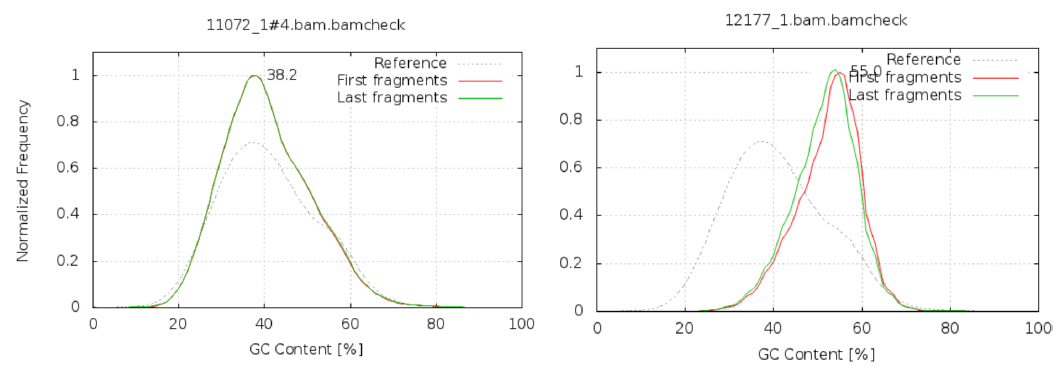
\includegraphics{img/gc_bias.png}
\caption{GC Content}
\end{figure}

    \hypertarget{gc-content-by-cycle}{%
\subsection{GC content by cycle}\label{gc-content-by-cycle}}

Looking at the GC content per cycle can help detect if the adapter
sequence was trimmed. For a random library, it is expected to be little
to no difference between the different bases of a sequence run, so the
lines in this plot should be parallel with each other like in the graph
on the left below. In the graph on the right, the initial spikes are
likely due to adapter sequences that have not been removed.

    \begin{figure}[!h]
\centering
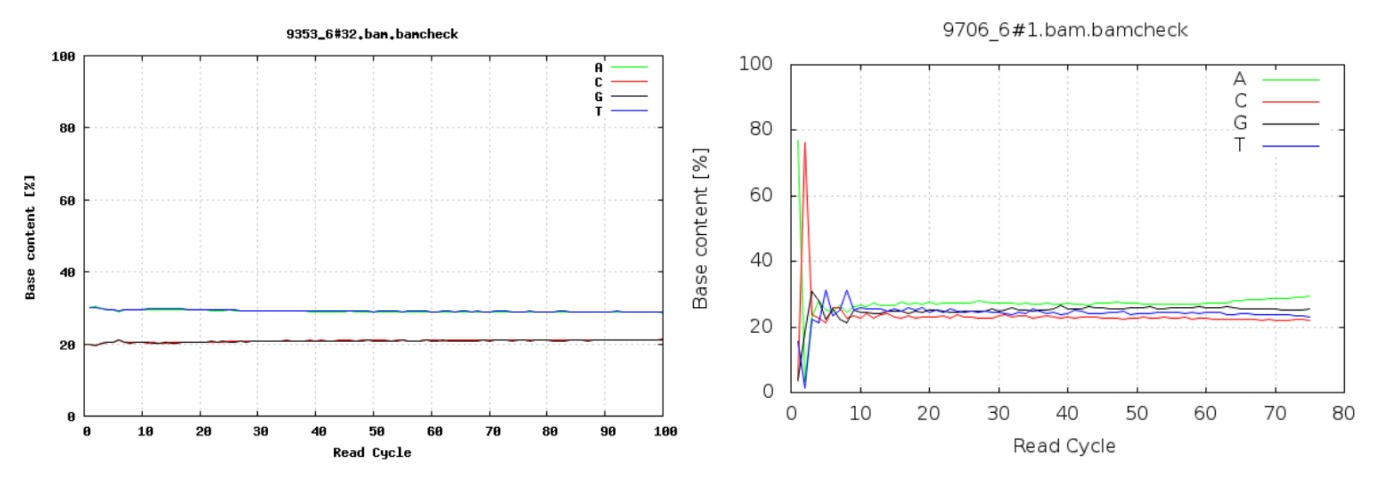
\includegraphics{img/acgt_per_cycle_comparison.png}
\caption{GC content by cycle}
\end{figure}

\pagebreak

    \hypertarget{fragment-size}{%
\subsection{Fragment size}\label{fragment-size}}

For paired-end sequencing the size of DNA fragments also matters. In the
first of the examples below, the fragment size peaks around 440 bp. In
the second however, there is also a peak at around 200 bp. This
indicates that there was an issue with the fragment size selection
during library prep.

    \begin{figure}[!h]
\centering
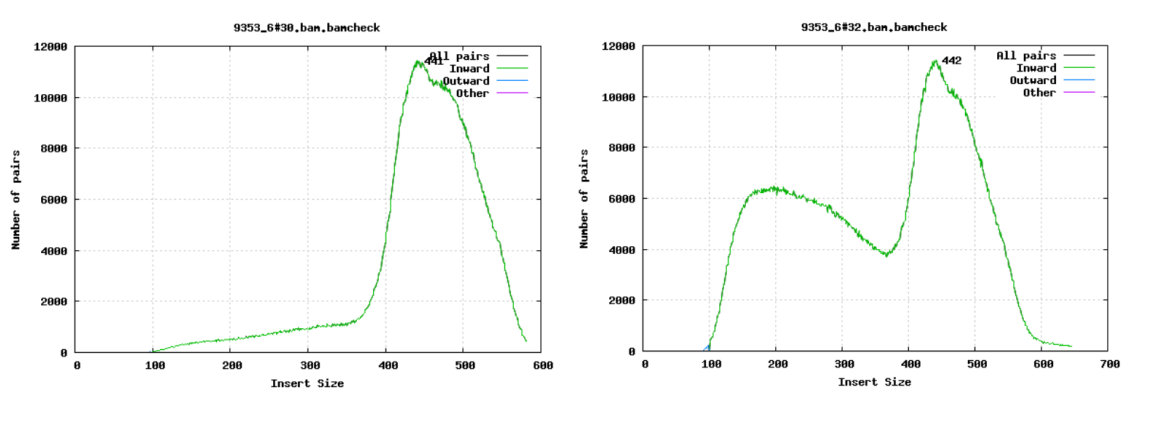
\includegraphics{img/fragment_size_comparison.png}
\caption{Fragment size distribution}
\end{figure}

    \hypertarget{exercises}{%
\subsubsection{Exercises}\label{exercises}}

\textbf{Q1: The figure below is from a 100bp paired-end sequencing. Can
you spot any problems?}

    \begin{figure}[!h]
\centering
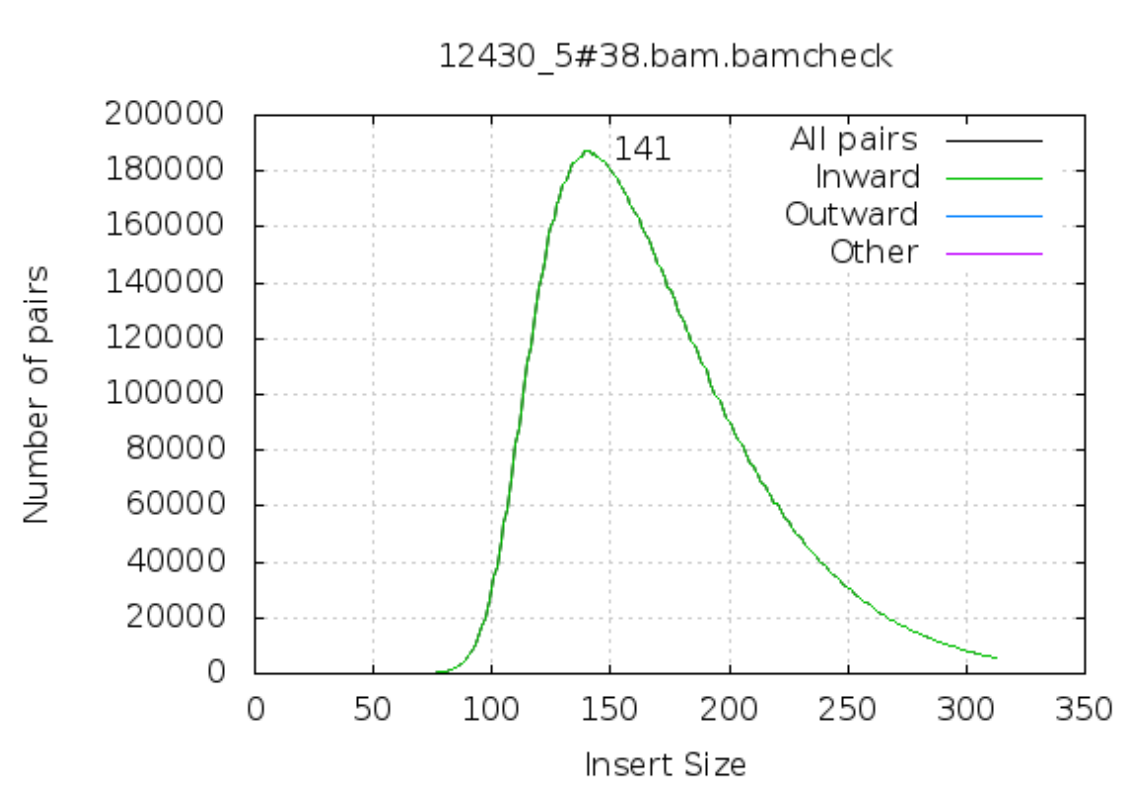
\includegraphics{img/insert_size_quiz.png}
\caption{Q1 Insert size distribution}
\end{figure}

    \hypertarget{insertionsdeletions-per-cycle}{%
\subsection{Insertions/Deletions per
cycle}\label{insertionsdeletions-per-cycle}}

Sometimes, air bubbles occur in the flow cell, which can manifest as
false indels. The spike in the right image provides an example of how
this can look.

    \begin{figure}[!h]
\centering
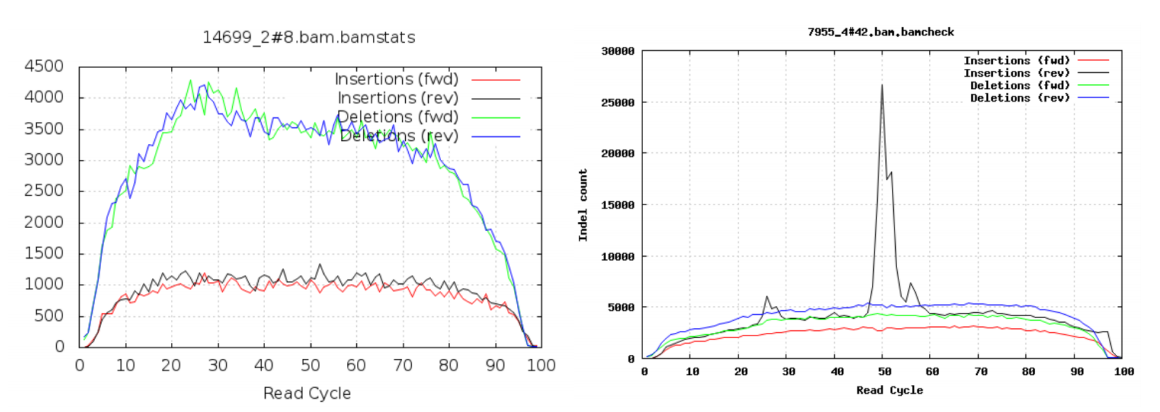
\includegraphics{img/indels_per_cycle_comparison.png}
\caption{Indels per cycle}
\end{figure}

    \hypertarget{generating-qc-stats}{%
\subsection{Generating QC stats}\label{generating-qc-stats}}

Now let's try this out! We will generate QC stats for two lanes of
Illumina paired-end sequencing data from yeast. The reads have already
been aligned to the
\href{ftp://ftp.ensembl.org/pub/current_fasta/saccharomyces_cerevisiae/dna}{Saccromyces
cerevisiae reference genome} to produce the BAM file lane1.sorted.bam.

    Now we will use \textbf{\texttt{samtools\ stats}} to generate the stats
for the primary alignments. The option \textbf{\texttt{-f}} can be used
to filter reads with specific tags, while \textbf{\texttt{-F}} can be
used to \textit{filter out} reads with specific tags. The following
command will include only primary alignments:

    \begin{tcolorbox}[breakable, size=fbox, boxrule=1pt, pad at break*=1mm,colback=cellbackground, colframe=cellborder]
\prompt{In}{incolor}{ }{\boxspacing}
\begin{Verbatim}[commandchars=\\\{\}]
samtools stats \PYZhy{}F SECONDARY data/lane1.sorted.bam \PY{l+s+se}{\PYZbs{}}
    \PYZgt{} data/lane1.sorted.bam.bchk
\end{Verbatim}
\end{tcolorbox}

    Have a look at the first 47 lines of the statistics file that was
generated:

    \begin{tcolorbox}[breakable, size=fbox, boxrule=1pt, pad at break*=1mm,colback=cellbackground, colframe=cellborder]
\prompt{In}{incolor}{ }{\boxspacing}
\begin{Verbatim}[commandchars=\\\{\}]
head \PYZhy{}n \PY{l+m}{47} data/lane1.sorted.bam.bchk
\end{Verbatim}
\end{tcolorbox}

    This file contains a number of useful stats that we can use to get a
better picture of our data, and it can even be plotted with
\textbf{\texttt{plot-bamstats}}, as you will see soon. First let's have
a closer look at some of the different stats. Each part of the file
starts with a \texttt{\#} followed by a description of the section and
how to extract it from the file. Let's have a look at all the sections
in the file:

    \begin{tcolorbox}[breakable, size=fbox, boxrule=1pt, pad at break*=1mm,colback=cellbackground, colframe=cellborder]
\prompt{In}{incolor}{ }{\boxspacing}
\begin{Verbatim}[commandchars=\\\{\}]
grep \PYZca{}\PY{l+s+s1}{\PYZsq{}\PYZsh{}\PYZsq{}} data/lane1.sorted.bam.bchk \PY{p}{|} grep \PY{l+s+s1}{\PYZsq{}Use\PYZsq{}}
\end{Verbatim}
\end{tcolorbox}

    \hypertarget{summary-numbers-sn}{%
\subsubsection{Summary Numbers (SN)}\label{summary-numbers-sn}}

This initial section contains a summary of the alignment and includes
some general statistics. In particular, you can see how many bases
mapped, and how much of the genome that was covered.

\hypertarget{exercises}{%
\subsubsection{Exercises}\label{exercises}}

    Now look at the output and try to answer the questions below.

\textbf{Q2: What is the total number of reads?}

    \begin{tcolorbox}[breakable, size=fbox, boxrule=1pt, pad at break*=1mm,colback=cellbackground, colframe=cellborder]
\prompt{In}{incolor}{ }{\boxspacing}
\begin{Verbatim}[commandchars=\\\{\}]

\end{Verbatim}
\end{tcolorbox}

    \textbf{Q3: What proportion of the reads were mapped?}

    \begin{tcolorbox}[breakable, size=fbox, boxrule=1pt, pad at break*=1mm,colback=cellbackground, colframe=cellborder]
\prompt{In}{incolor}{ }{\boxspacing}
\begin{Verbatim}[commandchars=\\\{\}]

\end{Verbatim}
\end{tcolorbox}

    \textbf{Q4: How many pairs were mapped to a different chromosome?}

    \begin{tcolorbox}[breakable, size=fbox, boxrule=1pt, pad at break*=1mm,colback=cellbackground, colframe=cellborder]
\prompt{In}{incolor}{ }{\boxspacing}
\begin{Verbatim}[commandchars=\\\{\}]

\end{Verbatim}
\end{tcolorbox}

    \textbf{Q5: What is the insert size mean and standard deviation?}

    \begin{tcolorbox}[breakable, size=fbox, boxrule=1pt, pad at break*=1mm,colback=cellbackground, colframe=cellborder]
\prompt{In}{incolor}{ }{\boxspacing}
\begin{Verbatim}[commandchars=\\\{\}]

\end{Verbatim}
\end{tcolorbox}

    \textbf{Q6: How many reads were paired properly?}

    \begin{tcolorbox}[breakable, size=fbox, boxrule=1pt, pad at break*=1mm,colback=cellbackground, colframe=cellborder]
\prompt{In}{incolor}{ }{\boxspacing}
\begin{Verbatim}[commandchars=\\\{\}]

\end{Verbatim}
\end{tcolorbox}

    \hypertarget{generating-qc-plots}{%
\subsubsection{Generating QC plots}\label{generating-qc-plots}}

Finally, we will create some QC plots from the output of the stats
command using the command \textbf{plot-bamstats} which is included in
the samtools package:

    \begin{tcolorbox}[breakable, size=fbox, boxrule=1pt, pad at break*=1mm,colback=cellbackground, colframe=cellborder]
\prompt{In}{incolor}{ }{\boxspacing}
\begin{Verbatim}[commandchars=\\\{\}]
plot\PYZhy{}bamstats \PYZhy{}p data/lane1\PYZhy{}plots/ data/lane1.sorted.bam.bchk
\end{Verbatim}
\end{tcolorbox}

    Now in your web browser open the file lane1-plots/index.html to view the
QC information.

\textbf{Q7: How many reads have zero mapping quality?}

    \begin{tcolorbox}[breakable, size=fbox, boxrule=1pt, pad at break*=1mm,colback=cellbackground, colframe=cellborder]
\prompt{In}{incolor}{ }{\boxspacing}
\begin{Verbatim}[commandchars=\\\{\}]

\end{Verbatim}
\end{tcolorbox}

    \textbf{Q8: Which read (forward/reverse) of the first fragments and
second fragments are higher base quality on average?}

    \begin{tcolorbox}[breakable, size=fbox, boxrule=1pt, pad at break*=1mm,colback=cellbackground, colframe=cellborder]
\prompt{In}{incolor}{ }{\boxspacing}
\begin{Verbatim}[commandchars=\\\{\}]

\end{Verbatim}
\end{tcolorbox}

    \textbf{Congratulations} you have reached the end of the Data formats
and QC tutorial!


    % Add a bibliography block to the postdoc



\end{document}
